% !TeX root = ../thuthesis-example.tex



\chapter{可预测预训练--性能可预测训练}

前面介绍了可预测预训练的训练策略部分。在使用包括超参数可预测扩展、基于新型学习率调度的可预测扩展的预训练方案之后,本文已经可以准确地预测不同模型规模和数据规模下的训练损失。然而即便如此,对于可预测预训练的目标而言,这也仅给出了不完整的答案。优化损失的确会随着模型规模的增加而按预期下降,这与大家熟知的大模型扩展定律相符;但学术界尚未建立关于下游任务性能(后简称性能或任务)的扩展定律。实际上,在模型规模的扩展过程中,性能远非可预测的。性能通常在小模型上提升较小,直到模型超过某个规模阈值后才会显著提升,这就是所谓 “涌现能力” 的典型表现。在本章中,我将深入研究这一现象,力图在”性能涌现“的背景下,建立起性能的平滑扩展定律。具体而言,我发现小模型尽管性能提升幅度较小,但展现出关键且持续的任务性能改进,由于测量分辨率不足,传统评估策略未能捕捉到这些改进。为了衡量这种改进,本章引入了 “PassUntil”评估策略,这是一种在解码阶段通过大量采样实现理论上无限分辨率的评估策略。借助 “PassUntil”,我对任务性能的扩展定律进行了定量研究。该研究包含两个部分。首先,我确定了一种严格的 “任务扩展定律”,这超过了学术届对于任务性能不可预测的认知。本文能够在训练开始前预测24亿参数模型在代码生成任务上的性能,偏差仅为0.05\%。其次,基于 “PassUntil”,本文对涌现能力进行了定量研究。我识别出一种 “加速涌现”,其扩展曲线无法用标准扩展定律函数拟合,且增长速度不断加快。然后我检验了两个假设,并暗示 “多回路假设” 可能是导致加速涌现的原因。 本章将详细介绍基于 “PassUntil”方法的性能可预测预训练。

\section{背景}
\subsection{损失连续性与性能突变性的矛盾}

大语言模型令人瞩目的成功在很大程度上依赖于扩大模型参数和预训练数据量。一直以来的观察表明,当考虑一系列架构近乎相同的模型时,更大的模型规模以及更多的预训练语料库总能使训练损失降低。这一观察结果已在数学上被形式化为损失扩展定律 \citep{kaplan2020scaling, henighan2020scaling}。该定律指出,模型在对数尺度下可降低的损失(L)与对数尺度下的模型规模(N)呈线性关系。扩展定律为大语言模型的科学扩展提供了指导,包括确定模型规模与预训练数据规模的平衡 \citep{hoffmann2022training, muennighoff2023scaling}。这将曾经略显盲目的扩展过程转变为一种有实证依据的方法。

然而,这种有益的扩展定律仅对损失做出预测,并未延伸到实际中遇到的真实任务性能。这种差异在全面的规模化方法中造成了巨大的差距 \citep{ganguli2022predictability}。

\begin{figure}[!htbp]
        \centering
        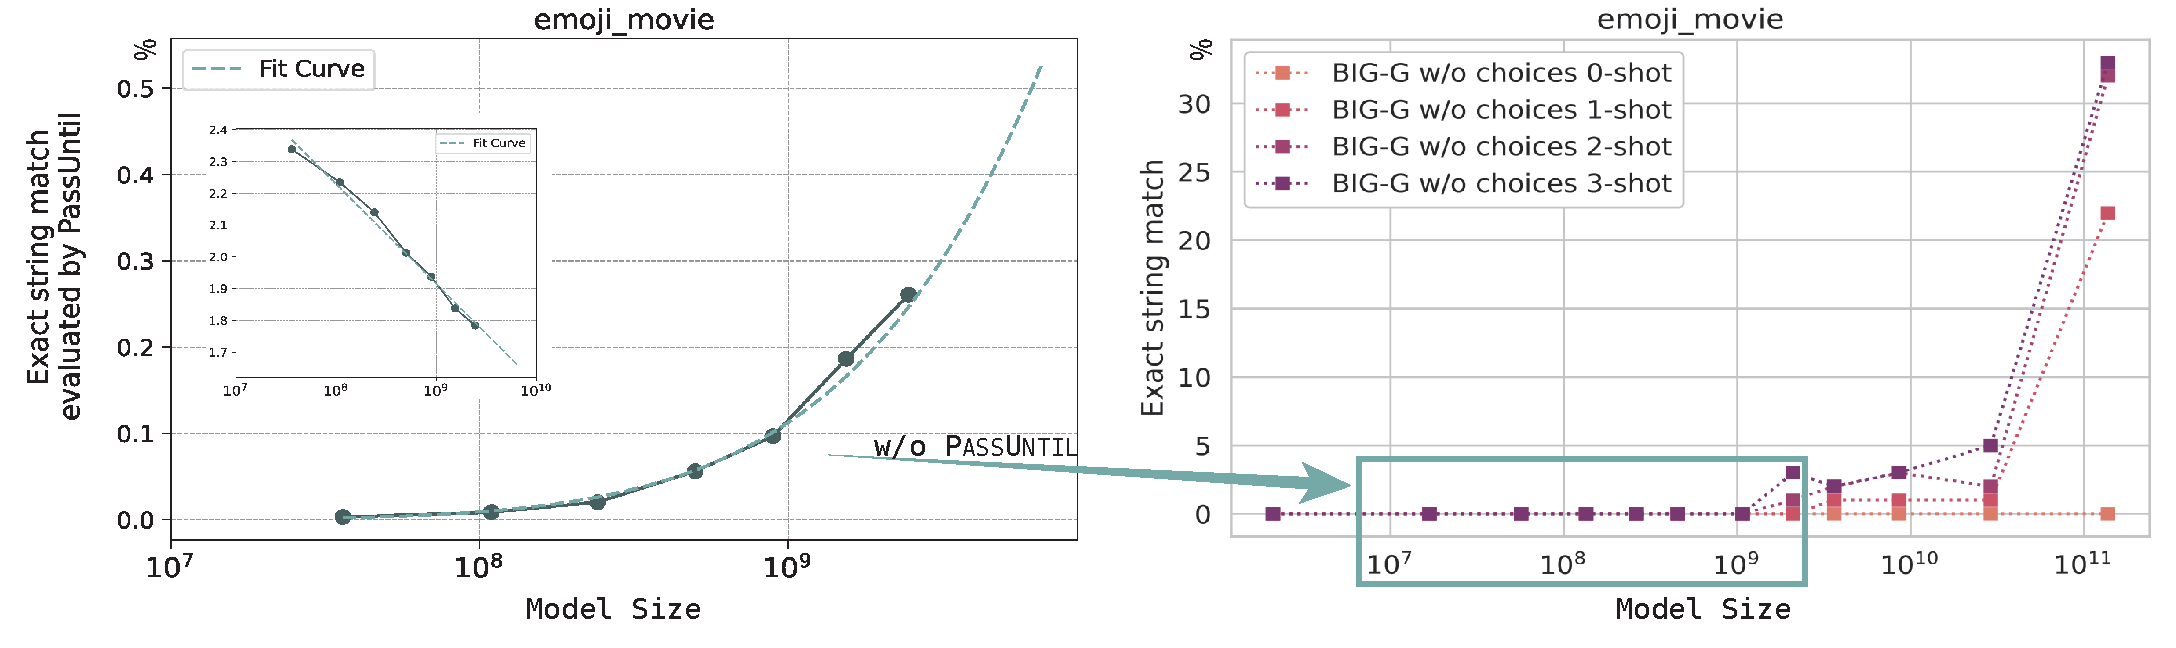
\includegraphics[width=\linewidth]{pufigs/themegraph.pdf}
    \caption{本章节的方法能够辨别出细微的性能提升(左图),而传统方法将其评估为全零(右图)。右图直接采用了 \citet{sorscher2022beyond} 中图9(a) 作为对比。该论文作者用此图来说明任务性能中的 “涌现” 行为。左图中的内嵌图展示了在 $\log(-\log(\cdot))$ 空间中的性能,呈现出很强的线性关系,支持任务扩展定律(公式(\ref{eq:task_scaling_raw}))。}
    \label{fig:themefig}
\end{figure}

将损失扩展定律扩展到任务性能的挑战主要源于扩展过程中任务性能的 “不连续性”。小于一定规模的语言模型表现出微不足道的性能,即在多项选择题中表现为随机猜测或在生成任务中获得零分。然而,当模型规模超过某个阈值时,性能会出现明显的激增,从而带来显著的非平凡性能。这种现象被总结为 “涌现能力” \citep{srivastava2022beyond, wei2022emergent}。这种涌现能力在各种模型系列和任务中都有观察到。似乎模型规模大小 内部发生了质的变化,使得模型开始展现出独特的能力。

虽然这些涌现现象表明大语言模型正在变得更强,但它们使任务性能的预测变得复杂。于是一个关键问题出现了:\textbf{能否从这些明显的不连续性中寻找出任务性能的可预测扩展规律?} 本文假设,从微不足道到卓越性能的这种看似不连续的现象,可能源于有限的评估分辨率。这里的 “分辨率”的意思是:当将评估视为对完成任务真实概率的一种度量时,某种评估策略的分辨率是该评估策略能够检测到的最小概率差异。通过采用更精细的分辨率,有可能揭示任务的扩展定律。 

与本章最相关的工作是 \citet{schaeffer2023emergent},它提出了两种使涌现能力连续化的方法,即 “改变度量” 和通过扩大测试集规模 “提高分辨率”。本文动机与 \citet{schaeffer2023emergent} 的 “改变度量” 方法不同,他们的方法认为采用其他连续度量可能会导致涌现能力消失,而应该使用替代的平滑度量。但是,替代的平滑度量(例如分布距离)的一个局限性在于,它们对评估者直观感知的目标度量(例如完全字符串匹配)提供的洞察力和关联性不足。相比之下,我的方法以一种新颖的方式扩展了 “提高分辨率” 的方法,并且能直接给出对目标度量的估计。

\section{方法设计}
\subsection{增加随机采样数量的先导实验}
\label{sec:pilot}
我通过可视化提高评估分辨率对语言模型的影响来开启探索过程。我选择了四个开源的小模型,并在BigBench任务的两个子集\citep{srivastava2022beyond}:“表情电影”(Emoji Movie)和“日期理解”(Date Understanding)上对它们进行评估。子集详情见\improvement{加上链接}。在解码过程中,我采用束搜索(Beam Search)和随机采样(采样次数分别为1次、100次和10000次)。如果一个测试实例有任何采样答案被评估为正确,那么该实例就被标记为“通过”。图\ref{tab:opensourcemodel_rs}中展示了“通过”的实例数量。

\begin{figure}[htbp]
\centering
    % \begin{tabular}{c|cccc|cccc}
    %     \toprule
    %   \multirow{2}{*}{\textbf{模型}}  & \multicolumn{4}{c|}{\textbf{表情电影}} & \multicolumn{4}{c}{\textbf{日期理解}}\\
    % \cline{2-9}
    %    & \textbf{束搜索} & \textbf{随机采样1次} & \textbf{随机采样100次} & \textbf{随机采样10000次}  & \textbf{束搜索} & \textbf{随机采样1次} & \textbf{随机采样100次} & \textbf{随机采样10000次}  \\
    %     \midrule
    %  Pythia - 410M & 0/41 & 0/41 & 2/41 & 31/41 & 0/50 & 0/50 & 8/50 & 42/50 \\
    %   Pythia - 1.4B & 0/41 & 0/41 & 7/41 & 38/41 & 2/50 & 2/50 & 18/50 & 46/50 \\
    %   OPT - 350M & 0/41 & 0/41 & 4/41 & 33/41 & 1/50 & 0/50 & 4/50 & 37/50 \\
    %   OPT - 1.3B & 0/41 & 0/41 & 12/41 & 39/41 & 1/50 & 1/50 & 12/50 & 46/50 \\
    %    \bottomrule
    % \end{tabular}
    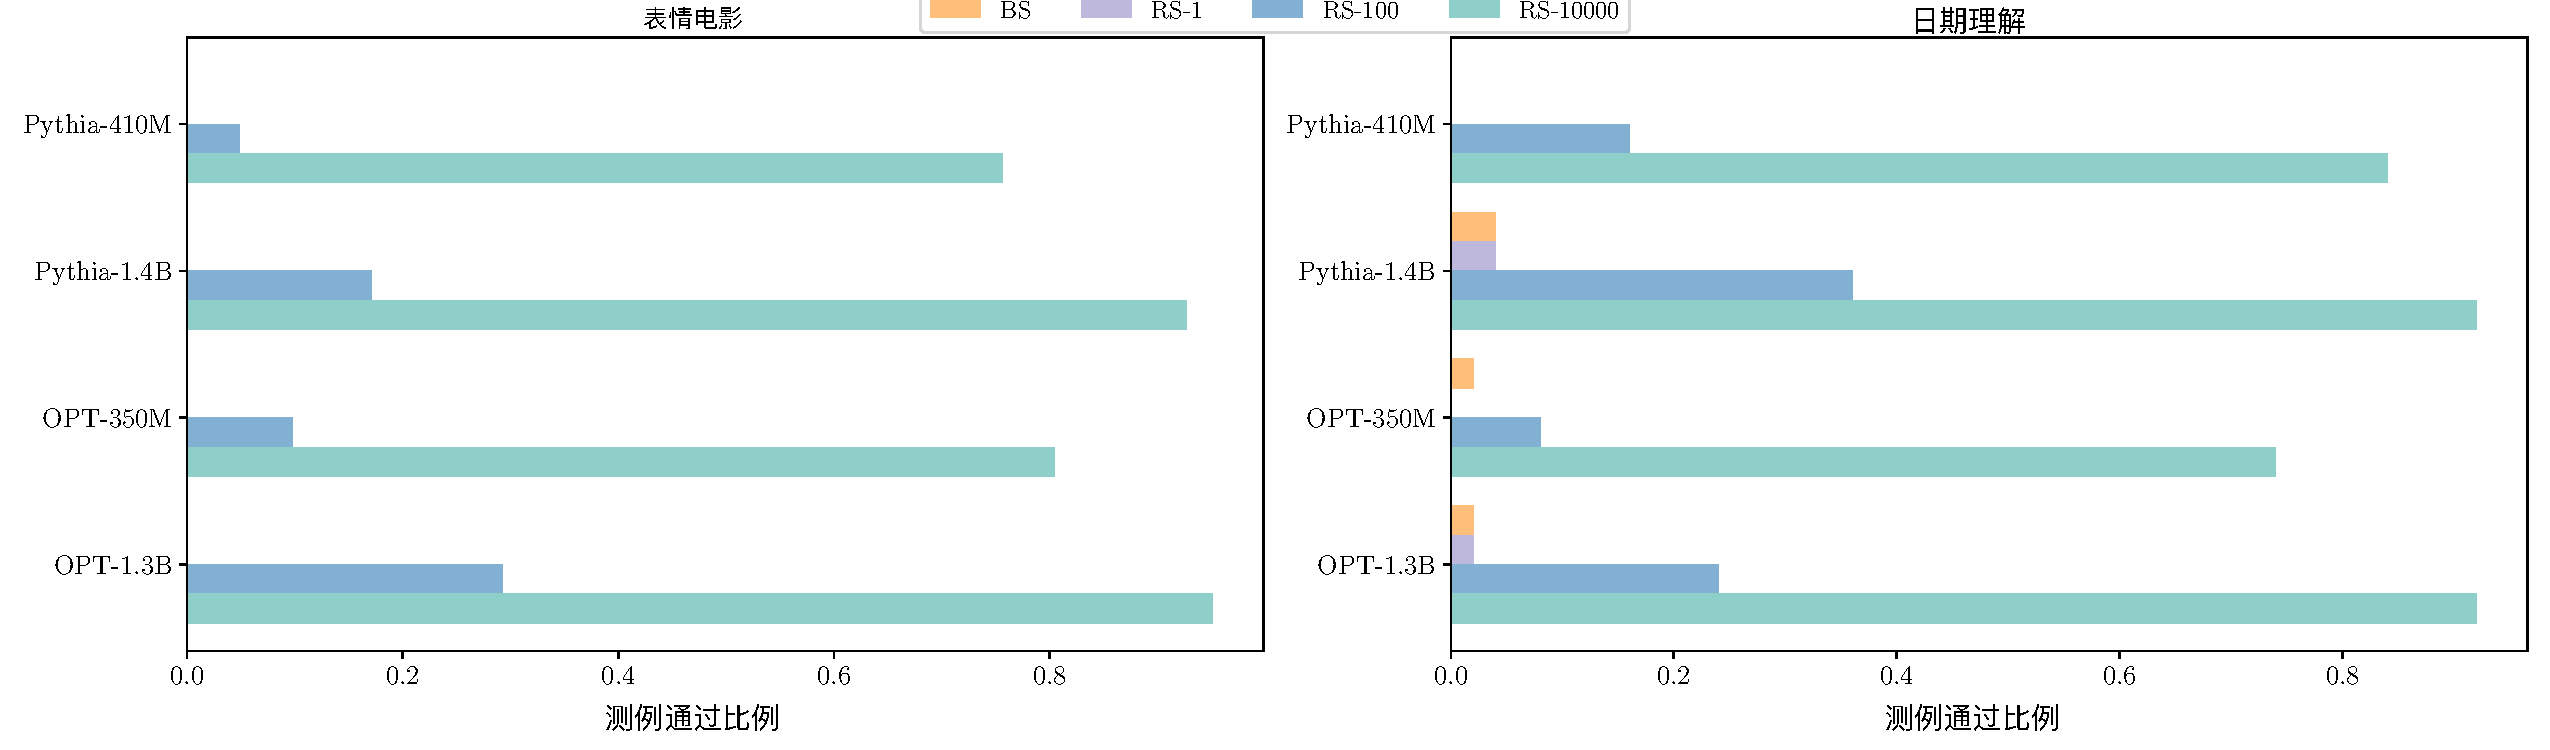
\includegraphics[width=0.98\textwidth]{pufigs/pilot-exp-fig.pdf}
    \caption{BS表示束搜索,RS-$K$表示随机采样$K$次。}
    \label{tab:opensourcemodel_rs}
\end{figure}

可以看到,即使对于这些给小模型带来较大难度的任务,在足够的随机采样次数下,大多数实例都能通过,这将有助于实现细微的任务性能增加。受此观察结果的启发,我提出以提高评估分辨率为核心的评估策略。首先是评估策略“PassUntil”,其次是实例级扩展曲线拟合,此外还有基于损失扩展定律推导出任务扩展定律。 接下来我将具体介绍提高评估分辨率的方法。

\subsection{“PassUntil”实现无限分辨率}
我将任务性能评估视为对模型通过某项任务概率的度量。注意,此处“通过”的定义不一定是要生成和标准答案字符串完全匹配的答案。例如,假设要预测模型在AlpacaEval\citep{alpaca_eval}上的性能,可以将“通过”定义为模型生成的内容优于GPT-4生成的内容。因此,“通过”的定义具有广泛的适用性。给定一个任务实例$s$,假设模型通过它的概率为$P(s)$,现在就是需要估计$\mathbb{E}_s[P(s)]$。随机采样固定次数$K$可以估计$P(s)$。然而,通常很难确定一个在计算上可接受,同时对于$P(s)$较小的困难样本又有足够分辨率的采样次数$K$。我提出“PassUntil”策略,即在生成一个答案后立即进行评估,在采样下一个生成结果之前确定该答案是否通过。持续采样,直到有$r$(一个预先确定的常数)个样本通过评估,并记录采样次数$K$。将$P(s)$的估计值称为“PassUntil”分数$\textsc{PU}$,其定义为:
\begin{equation}
\label{equ:pudef}
    \textsc{PU} = \frac{r}{K}
\end{equation}
从理论上讲,$\textsc{PU}$能够测量极小的成功率。

“PassUntil”具有以下性质。
\begin{theorem}
$\textsc{PU}$是$P(s)$的最大似然估计。
\end{theorem}

\begin{proof}
失败次数$f = K - r$服从成功概率为$P(s)$的负二项分布。而$r/K$是$P(s)$的最大似然估计。
\end{proof}


在实际应用中,考虑到评估效率,我将$r$设置得尽可能小,如$1$。我还将$K$的上限设置为一个较大的数,如$10^5$,以防止在遇到极低的$P(s)$时进行无休止的采样。需要注意的是,许多实例在达到这个上限之前就停止采样了。接下来我将讨论“PassUntil”的必要性和局限性。

\begin{enumerate}
    \item \textbf{必要性}。 一般来说,从理论上根据真实解的词元概率推导出$P(s)$是不可行的。这主要有两个原因:第一,可能存在多个可行解;第二,即使只有一个解,除了最优分词方式外,还有多种解码方式可以解码出该解。例如,在GPT-4的“cl100k-base”词表中,用token序列[4513]、[717,18]和[16,17,18]都可以解码为字符串“123”,这导致标准答案在词元层面并不一定是唯一的,进一步导致通过计算词元概率来得到任意的目标观测指标是不可行的。
    \item \textbf{局限性(1)。} 目前,本文的评估策略设计适用于随机预测的基线能取得0分的得分的目标指标,即$P(s) = 0$的情况。在以多项选择得分作为评估指标的情况下,相对于模型的真实性能,评估结果往往会出现偏高的偏差(例如,对于四个选项的题目,随机猜测的$P(s) = 0.25$)。这种随机噪声可能会掩盖较小模型所取得的改进。对于具有非零随机基线的任务扩展定律的探索仍然是未来研究的课题。
    \item \textbf{局限性(2)。} 由于随机采样在大语言模型中广泛使用,目前本文仅将其视为一种可行的目标解码策略。将束搜索作为目标解码策略及其与随机采样的关系,为未来的探索和研究提供了一个有趣的方向。 
\end{enumerate}


\subsection{任务扩展定律}
接着,我推导出“PassUntil”所遵循的任务扩展定律。假设生成下一个词元的测试损失按照公式(\ref{eq:loss_scaling_law})的扩展定律下降,则“PassUntil” 将可以用如下规律理论推出:
\begin{equation}
\label{eq:task_scaling_raw}
    \textsc{PU} \sim \prod_{i=1}^{|y|} P(y_i|\{x_{1:|x|}, y_{1:i - 1}\}) = \prod_{i=1}^{|y|} \exp(-{c_i}{{N}^{-\alpha_i}} - L_{0i}),
\end{equation}
其中,$x_{1:|x|}$是输入序列,$y_{1:|y|}$是解码出正确答案的最可能序列(假设相较于其他序列,它占主导地位)。
假设给定一个足够强大的大语言模型(LLM),测试样本是可通过的,那么每个词元的不可约损失$L_{0i}$趋近于$0$。并且假设答案中每个词元的测试损失在扩展时以均匀的速度下降(即$\forall i$,$a_i = a$),可以推导出关于任务性能的$\textsc{PU}$的以下函数:
\begin{equation}
\label{eq:exp_scaling}
    \textsc{PU}(c, \alpha; N) \sim \operatorname{exp}(\sum_i -{c_i}{{N}^{-\alpha}} ) = \operatorname{exp}(-{c}{{N}^{-\alpha}})
\end{equation}
其中$c = \sum_i c_i$。值得指出的是,尽管方式不同,但是得到的数学模型与GPT-4技术报告\citep{openai2023gpt4}以及\citet{schaeffer2023emergent}中的公式(4)有共同点。

\subsection{拟合策略}
\textbf{数据集层面的拟合。}在拟合$\textsc{PU}$中的参数$c$、$\alpha$时,数据集层面的拟合是可行的。对于扩展曲线中的第$j$个模型(其参数量大小为$N_j$),首先在测试集上对单个测试样本的$\textsc{PU}$求平均,得到$\operatorname{log}(-\operatorname{log}(\textsc{PU}(N_j)))$,然后对$\operatorname{log}N_j$进行线性回归。

\textbf{实例(instance)层面的拟合。}
\label{sec:instance_level_pass}
本文注意到,测试数据集中不同测试实例(instance,或者称作样本)之间的差异会导致不同的扩展行为。这意味着当测试集内,不同实例的难度不同时,数据集层面的拟合可能不准确。例如,简单问题的$\textsc{PU}$在小模型上就会很快饱和到$1$,而难题仍然表现出微不足道的性能。因此本文进一步提出实例层面的拟合方法:为每个实例拟合一个单独的“PassUntil”分数, 即Instance-level PassUntil($\textsc{IPU}$),并将它们汇总以估计整个数据集的情况。即,假设数据集为$S = \{s\}$, 每个测试实例对应的IPU参数为$c_s, a_s$, 则:
\begin{equation}
    {\textsc{PU}}(\{c_s, a_s\}; N) = \frac{1}{|S|}\sum_s {\operatorname{IPU}}(c_s, a_s; N)
\end{equation}


\section{可预测扩展实验}

在本节中,我将展示所提出的框架在实际实验中的作用。我预训练了两个系列的语言模型,参数规模从3000万(0.03B)到24亿(2.4B)不等。基于系列中其他模型的性能来预测24亿参数模型的性能。

\subsection{实验配置}
\label{sec:train}
\subsubsection{模型配置}
在扩大Transformer模型规模时,需要保持其 “形状” 一致。对于扩展曲线中的第\(i\)个模型,将层数设置为\(4i\),注意力头的数量设置为\(\lfloor \frac{i(8 + i)}{4} \rfloor\),头的维度设置为\(64\)。这使得隐藏状态的维度\(d_m\)为\(d_hn_h\)。我将前馈层的维度设置为\(2.5d_m\)。具体数值列于表\ref{tab:pu_model_configs}中的模型配置里。该架构与LLaMA类似\citep{touvron2023llama}。一些细微差异包括:我在输入和输出嵌入之间使用共享嵌入,并且使用门控高斯误差线性单元(gated-GeLU)\citep{hendrycks2016gaussian} 替代门控SiLU\citep{DBLP:journals/corr/abs-2002-05202}。

\begin{table}[htbp]
    \centering
    \caption{扩展曲线中各模型的模型配置和训练配置。N(十亿)表示模型的非嵌入参数数量,单位为十亿。BS(百万)表示用于训练模型的每个批次中的令牌数(即批量大小),单位为百万。TS表示训练步数。令牌数(十亿)指用于训练模型的令牌总数。}
\scalebox{0.9}{
    \begin{tabular}{c|cccccccccc}
    \toprule
        名称 & i & N(十亿)& $d_m$ & $d_{ff}$ & $d_h$ & $n_h$ & $L$ & BS(百万) & TS & 词元数(十亿)\\
    \midrule
  $\backslash$ & i & $\backslash$ & $d_hn_h$ & $2.5d_{m}$ & 64 & $\lfloor \frac{i(8 + i)}{4} \rfloor$ & $\lfloor4i\rfloor$ & $\backslash$ & $\backslash$ & $\backslash$\\
           0.03B & 3 &  0.036 & 512 & 1280 & 64 & 8 & 12 & 0.33 & 2196 & 0.72\\
          0.1B & 4 & 0.109 & 768 & 1920 & 64 & 12 & 16  & 0.88 & 2464 & 2.18\\
         0.2B & 5 & 0.241 & 1024 & 2560 & 64 & 16 & 20  & 1.57 & 3064 & 4.82\\
        0.5B & 6 & 0.499 & 1344 & 3360 & 64 & 21 & 24 & 2.10 & 4758 & 9.99\\
        0.9B & 7 & 0.892 & 1664 & 4160 & 64 & 26 & 28  & 2.95 & 6049 & 17.9  \\
        1.5B & 8 & 1.542 & 2048 & 5120 & 64 & 32 & 32 & 4.26 & 7230 & 30.8\\
       2.4B & 9 & 2.45 & 2432 & 6080 & 64 & 38 & 36 & 5.51 & 8900 & 49.0\\
    \bottomrule
    \end{tabular}
}
    \label{tab:pu_model_configs}
\end{table}



\subsubsection{预训练语料库}
对于系列一,我在单目标任务(即代码生成任务)上进行评测, 因此使用单源预训练预料——StarCoder数据集\citep{li2023starcoder}——作为预训练数据。对于系列二,我在多目标任务上进行评测,使用StarCoder和Pile数据集\citep{gao2020pile}的混合数据。利用最优计算大语言模型的方法\citep{hoffmann2022training},我将每个模型规模的最大预训练词元数设置为\(20N\),其中\(N\)是模型的非嵌入参数数量。表\ref{tab:series1_data_mixture}和表\ref{tab:series2_data_mixture}分别展示了系列1和系列2大语言模型的具体数据混合比例。


\begin{table}
        \centering
        \caption{系列一模型的预训练语料。}
        \begin{tabular}{c|c}
        \toprule
           语料库   &  词元占比 \\
        \midrule
        StarCoder\_Python &  0.3\\
        StarCoder\_Others &  0.7\\
    \bottomrule
        \end{tabular}
        \label{tab:series1_data_mixture}
    \centering
\end{table}

\begin{table}
    \centering
    \caption{系列二模型的预训练语料}
    \begin{tabular}{c|c}
    \toprule
       语料库   &  词元占比 \\
    \midrule
    StarCoder\_Python &  0.15\\
    StarCoder\_Others &  0.12\\
    Stack\_Overflow & 0.03 \\
    Arxiv & 0.05 \\
    Pile & 0.65 \\
\bottomrule
    \end{tabular}
    \label{tab:series2_data_mixture}
\end{table}


\subsubsection{超参数设置}
\label{app:hyperparameters}
\textbf{学习率}:采用余弦退火学习率调度器,与之前的研究\citep{touvron2023llama, touvron2023llama2, hoffmann2022training}类似。在不同的模型规模下,最大学习率始终固定为\(0.01\),在此学习率下没有出现明显的损失爆炸情况。这种稳定性可能归因于前面几章提到的归一化策略\citep{yang2022tensor}以及跨规模增加的批量大小。如前文所述,与\citet{hoffmann2022training}的研究结果一致,我研究得到对于训练大语言模型直至特定的结束步数,余弦退火学习率调度器的最优循环长度应等于结束步数。偏离此最优循环长度,无论是变长还是变短,都会导致性能次优。

\textbf{批量大小}:为了估计模型预训练所需的最优批量大小,我按照\citet{kaplan2020scaling}的方法重复实验,以确定模型的最优批量大小,并在最优批量大小的基础上对实际批量大小进行微调,以最大化GPU利用率。批量大小和训练步数的值列于表\ref{tab:pu_model_configs}中。 

\subsubsection{测试集配置}
\label{app:testset}
在本小节中,我介绍实验中的测试集和评估细节。
\paragraph{HumanEval}
\label{app:humaneval}
OpenAI发布的HumanEval\citep{chen2021evaluating}数据集包含164个编程问题。每个问题由一个函数签名、一个文档字符串、一个函数体和多个单元测试组成。我对该数据集采用零样本方法进行评估。只有当大语言模型生成的代码成功通过所有单元测试时,才认为代码完成通过。在我的评估中,将“PassUntil”中的采样次数上限设置为\(10^4\)。

\paragraph{表情电影(Emoji Movie)}
\label{app:emoji_movies}
“表情电影”是评测集合BigBench\citep{srivastava2022beyond}中的一个子任务,要求大语言模型根据用表情符号描述的情节识别知名电影。评估方法结合了思维链(Chain-of-Thought,CoT)和四样本上下文学习。我从原始的50个实例中选择41个测试实例(剔除了9个干扰实例,详见章节\ref{app:removing_distracting})构成测试集,并任意指定4个实例作为少样本上下文。使用GPT-4为这些上下文样本的产生思维链,并期望模型能读取这四个上下文样本的思维链示例,对测试样本生成一段思考过程,然后给出答案。评估方法采用提取字符串匹配,即模型的输出包含目标电影名称。我将采样次数上限设置为\(10^5\)。 

\paragraph{日期理解}
\label{app:dateunderstanding}
“日期理解” 也是评测集合BigBench\citep{srivastava2022beyond}的一个子集,旨在通过提出与日期推理相关的问题,评估大语言模型理解日期的能力。
对于此任务的评估,我同样采用四样本上下文学习。从原始的50个实例中随机抽取47个实例组成测试集(剔除了3个干扰实例,详见章节\ref{app:removing_distracting})。从剩余数据集中随机抽取4个实例作为上下文示例。同样使用提取字符串匹配的方式来衡量大语言模型的输出,并将采样次数上限设置为\(10^5\)。

\paragraph{非自然上下文学习任务}
\label{app:unantural_in_context_learning}
非自然上下文学习任务是BigBench\citep{srivastava2022beyond}中一系列独特的子任务。这些子任务旨在评估模型在上下文序列被有意改变为可能超出训练数据分布的情况下进行上下文学习的能力,这要求模型关注非传统的上下文模式。表\ref{tab:unnaturalincontextexample}列举了这些子任务的一些实例。
对于每个任务,采用4样本上下文学习配置,从数据集中随机抽取20个实例组成测试集。从剩余数据集中随机选择4个实例作为上下文。我使用提取字符串匹配的方式来衡量大语言模型的输出,并将采样次数上限设置为\(10^5\)。

\begin{table}[!htbp]
    \centering
    \label{tab:unnaturalicl}
    \caption{非自然上下文学习任务中的示例任务}
    \begin{tabular}{p{4cm}l}
        \toprule
        \textbf{任务名称}  & \textbf{示例} \\
        \midrule
        日期  & 输入: 2015-10-22\ 目标: \textit{!10!22!2015!}\\
        非自然格式日期  & 输入:!08!24!1984!\ 目标: \textit{1984-08- 24}\\
        非自然内容日期  & 输入: 96980-49665-10674\ 目标: \textit{!49665!10674!96980!}\\
        非自然格式与内容日期  & 输入:!49665!10674!96980!\ 目标: \textit{96980-49665-10674}\\
        原样输出  & 输入: a, b, c, d, e\ 目标: \textit{a, b, c, d, e} \\
        反转自然内容  & 输入: t, u, o, b, a\ 目标: \textit{a, b, o, u, t} \\
        反转成自然内容  & 输入: r, o, o, m, s\ 目标: \textit{s, m, o, o, r}  \\
        两位数运算  & 输入: 10 - 10 =\ 目标: \textit{20}\\
        \bottomrule
    \end{tabular}
    \label{tab:unnaturalincontextexample}
\end{table}



\subsection{损失扩展定律验证}
图\ref{fig:loss_scaling}展示了各模型的训练损失曲线。显然,最终训练损失按照扩展定律下降。这些通过实证观察得到的损失扩展定律,为后续对任务性能的近似分析奠定了基础。需要注意的是,尽管15亿和24亿参数的模型出现了损失尖峰,但最终仍收敛到扩展定律,这体现了该经验定律的稳健性。


\begin{figure}[!htbp]
        \centering
        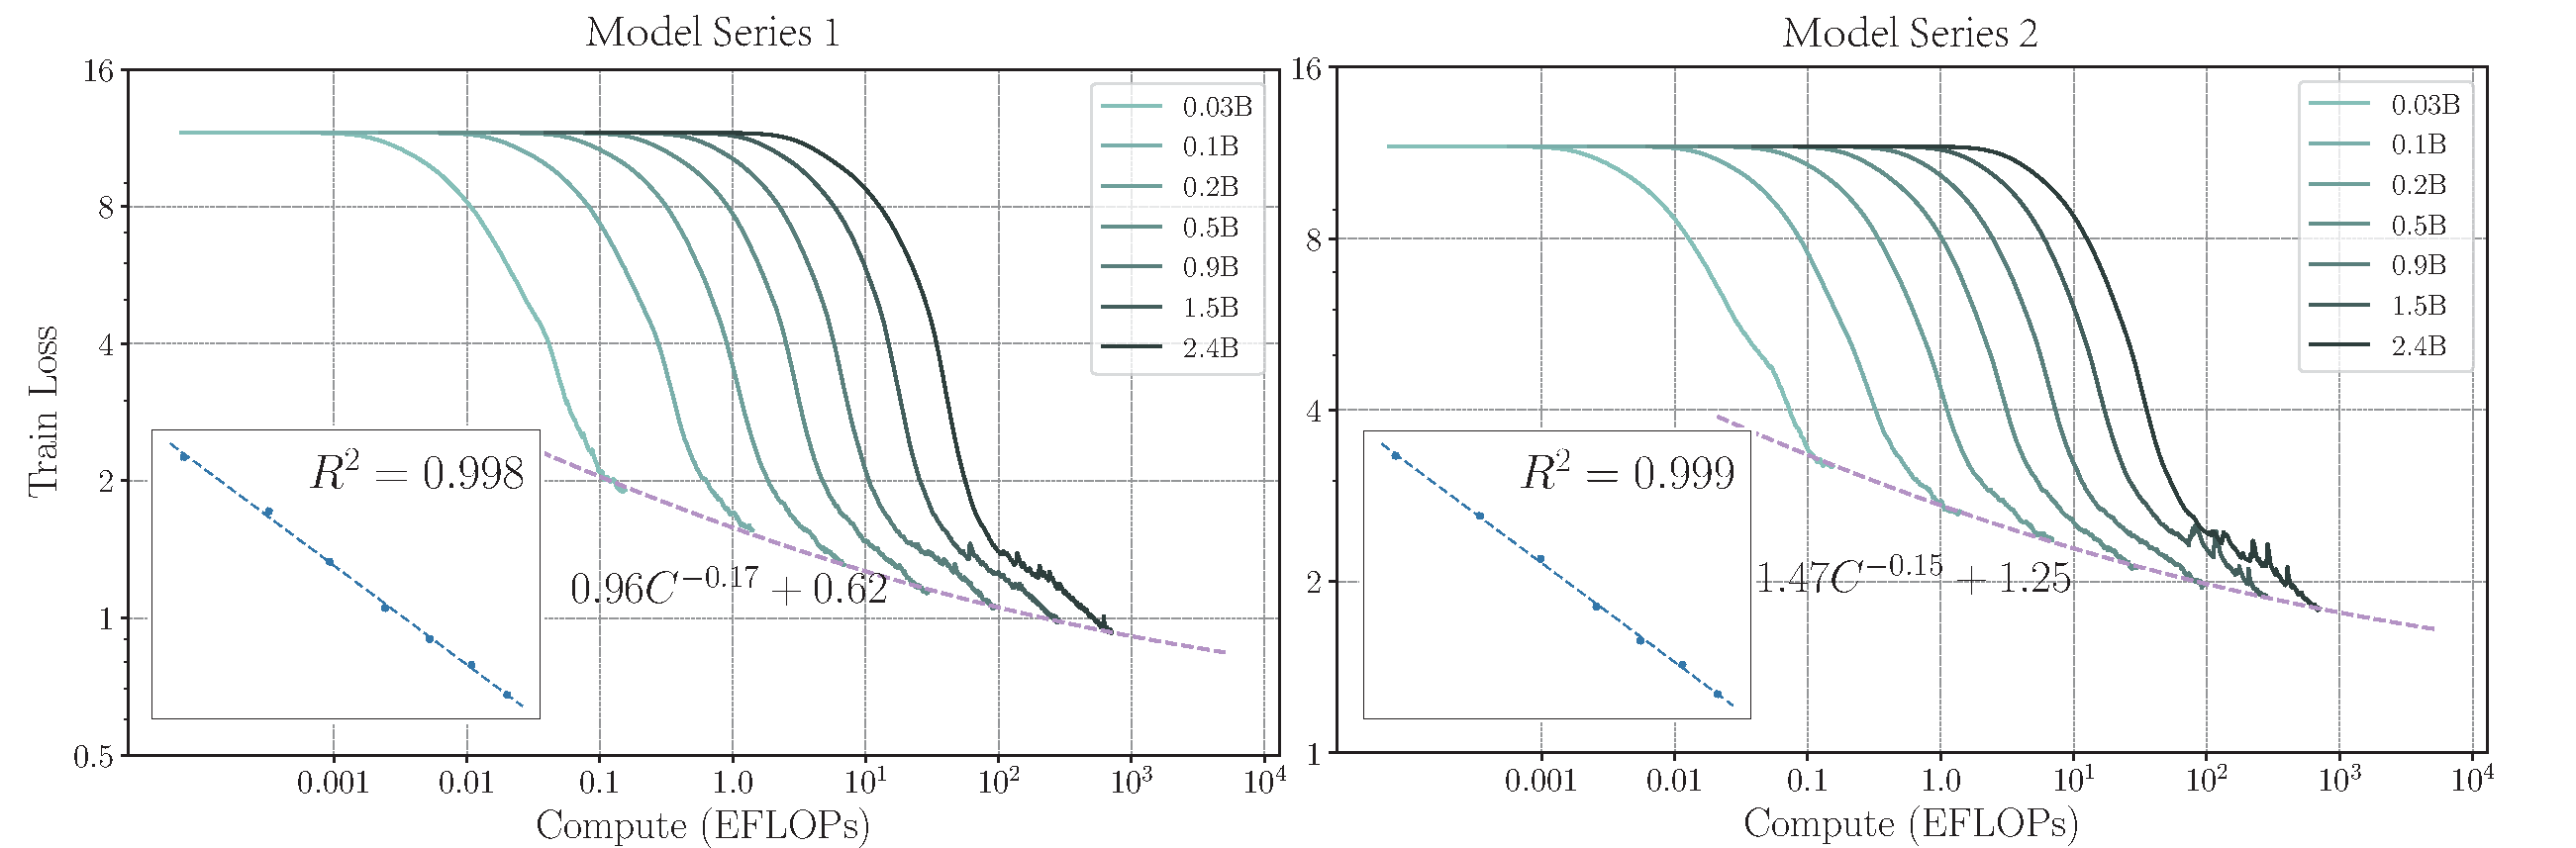
\includegraphics[width=0.85\linewidth]{pufigs/train_loss_2series.pdf}
        \label{fig:train_loss_2series}
\caption{在不同数据混合上训练的两个系列模型的训练损失。内插图展示了相对于模型规模的最终步骤可约损失,以对数尺度表示。 }
    \label{fig:loss_scaling}
\end{figure}



\subsection{去除干扰因素}
\label{app:removing_distracting}
我注意到,在测量模型规模扩展过程中的微小性能提升时,去除干扰因素至关重要。干扰因素指的是某个测试实例在所需能力或评估偏差方面与其他测试实例存在显著差异。请注意,我基于对测试实例的观察来选择干扰因素,这在预测24亿参数模型时不会导致信息泄露。

举例说明如下:对于“表情电影”任务,由于采用提取字符串匹配的评分方式,即模型答案是否正确取决于其输出中是否包含电影名称,而部分电影名称是常用词,这使得即使是规模较小的模型也能根据评估标准“猜出”正确答案。我找出了电影名字是常见单词或词组的实例,如图\ref{fig:emoji_common_words}所示,不同规模模型在这些实例上的通过率没有显著关联。换句话说,扩展定律对这些问题的模型性能影响不大。因此,将此类干扰因素排除在外就变得至关重要。我剔除了流行工具包NLTK识别出的常用词形式的电影名称\footnote{\url{https://www.nltk.org/}}。

对于“日期理解”任务,我省略了表\ref{tab:du_distracting}中所示的以下实例。这些实例仅要求模型从上下文中提取答案,而不要求对日期进行推理。这是和本文关心的目标能力是两种不同的能力,如果混杂在一起评测只会导致混乱的结论。

在GPT-4报告\citep{openai2023gpt4}中,他们将HumanEval数据集按不同难度分成单独的区间,并对每个区间进行扩展预测,从而消除了简单示例对困难示例的干扰。

\begin{table}[!htbp]
\centering
\caption{“日期理解”任务中的干扰实例。}
\scalebox{0.9}{
    \begin{tabular}{p{13cm}}
        \toprule
      \textbf{示例} \\
        \midrule
         今天的会议重新安排到明天上午11点,1924年10月16日。明天的日期(格式为MM/DD/YYYY)是什么? \\
         \hline
         昨天是1929年12月31日。今天不可能是1929年12月32日,因为12月只有31天。昨天的日期(格式为MM/DD/YYYY)是什么? \\
        \hline
        今天是9月7日。简正在观看2003年的美国国家橄榄球联盟(NFL)比赛。今天的日期(格式为MM/DD/YYYY)是什么? \\ 
    \bottomrule
    \end{tabular}
}
    % \label{tab:unnaturalicl}
    \label{tab:du_distracting}
\end{table}

\begin{figure}[h]
    \centering
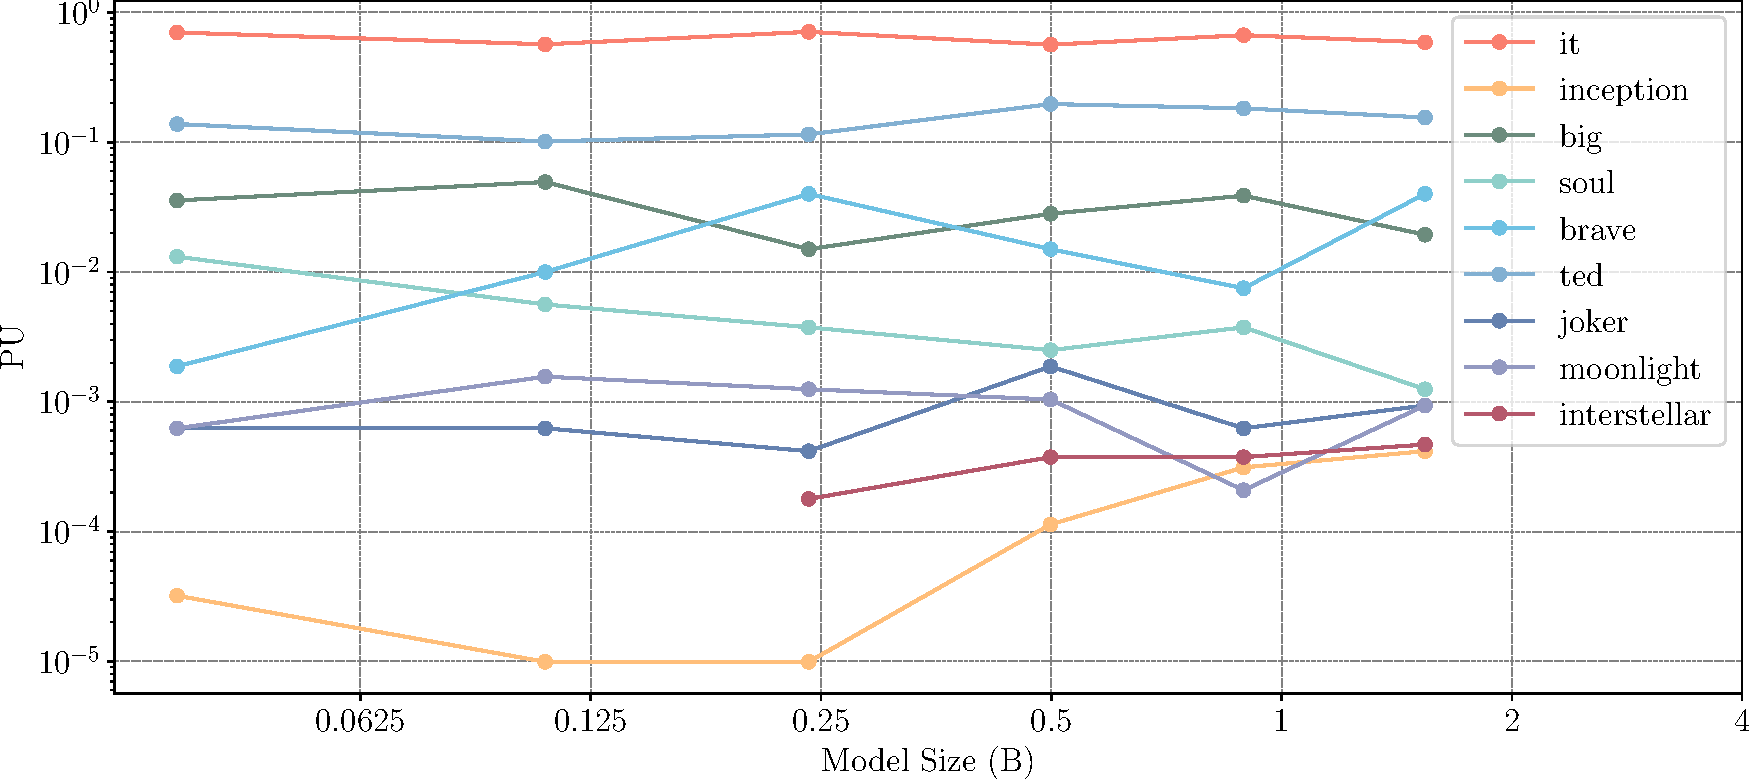
\includegraphics[width=0.85\linewidth]{pufigs/emoji_removing_distracting.pdf}
\caption{在这些实例上,大模型和小模型的 \textsc{PU} 相似(主要是因为从词汇空间中随机采样),这在实验中造成了干扰。}
    \label{fig:emoji_common_words}
\end{figure}



\subsection{数据集层面的拟合}
我选择了HumanEval\citep{chen2021evaluating}、“表情电影”(Emoji Movie)以及“日期理解”(Date Understanding)\citep{srivastava2022beyond}作为评估任务。
需注意,“表情电影” 通常被视为 “涌现能力” 的代表\citep{srivastava2022beyond}(见图\ref{fig:themefig}中的右图)。


\begin{figure}[!htbp]
        \centering
        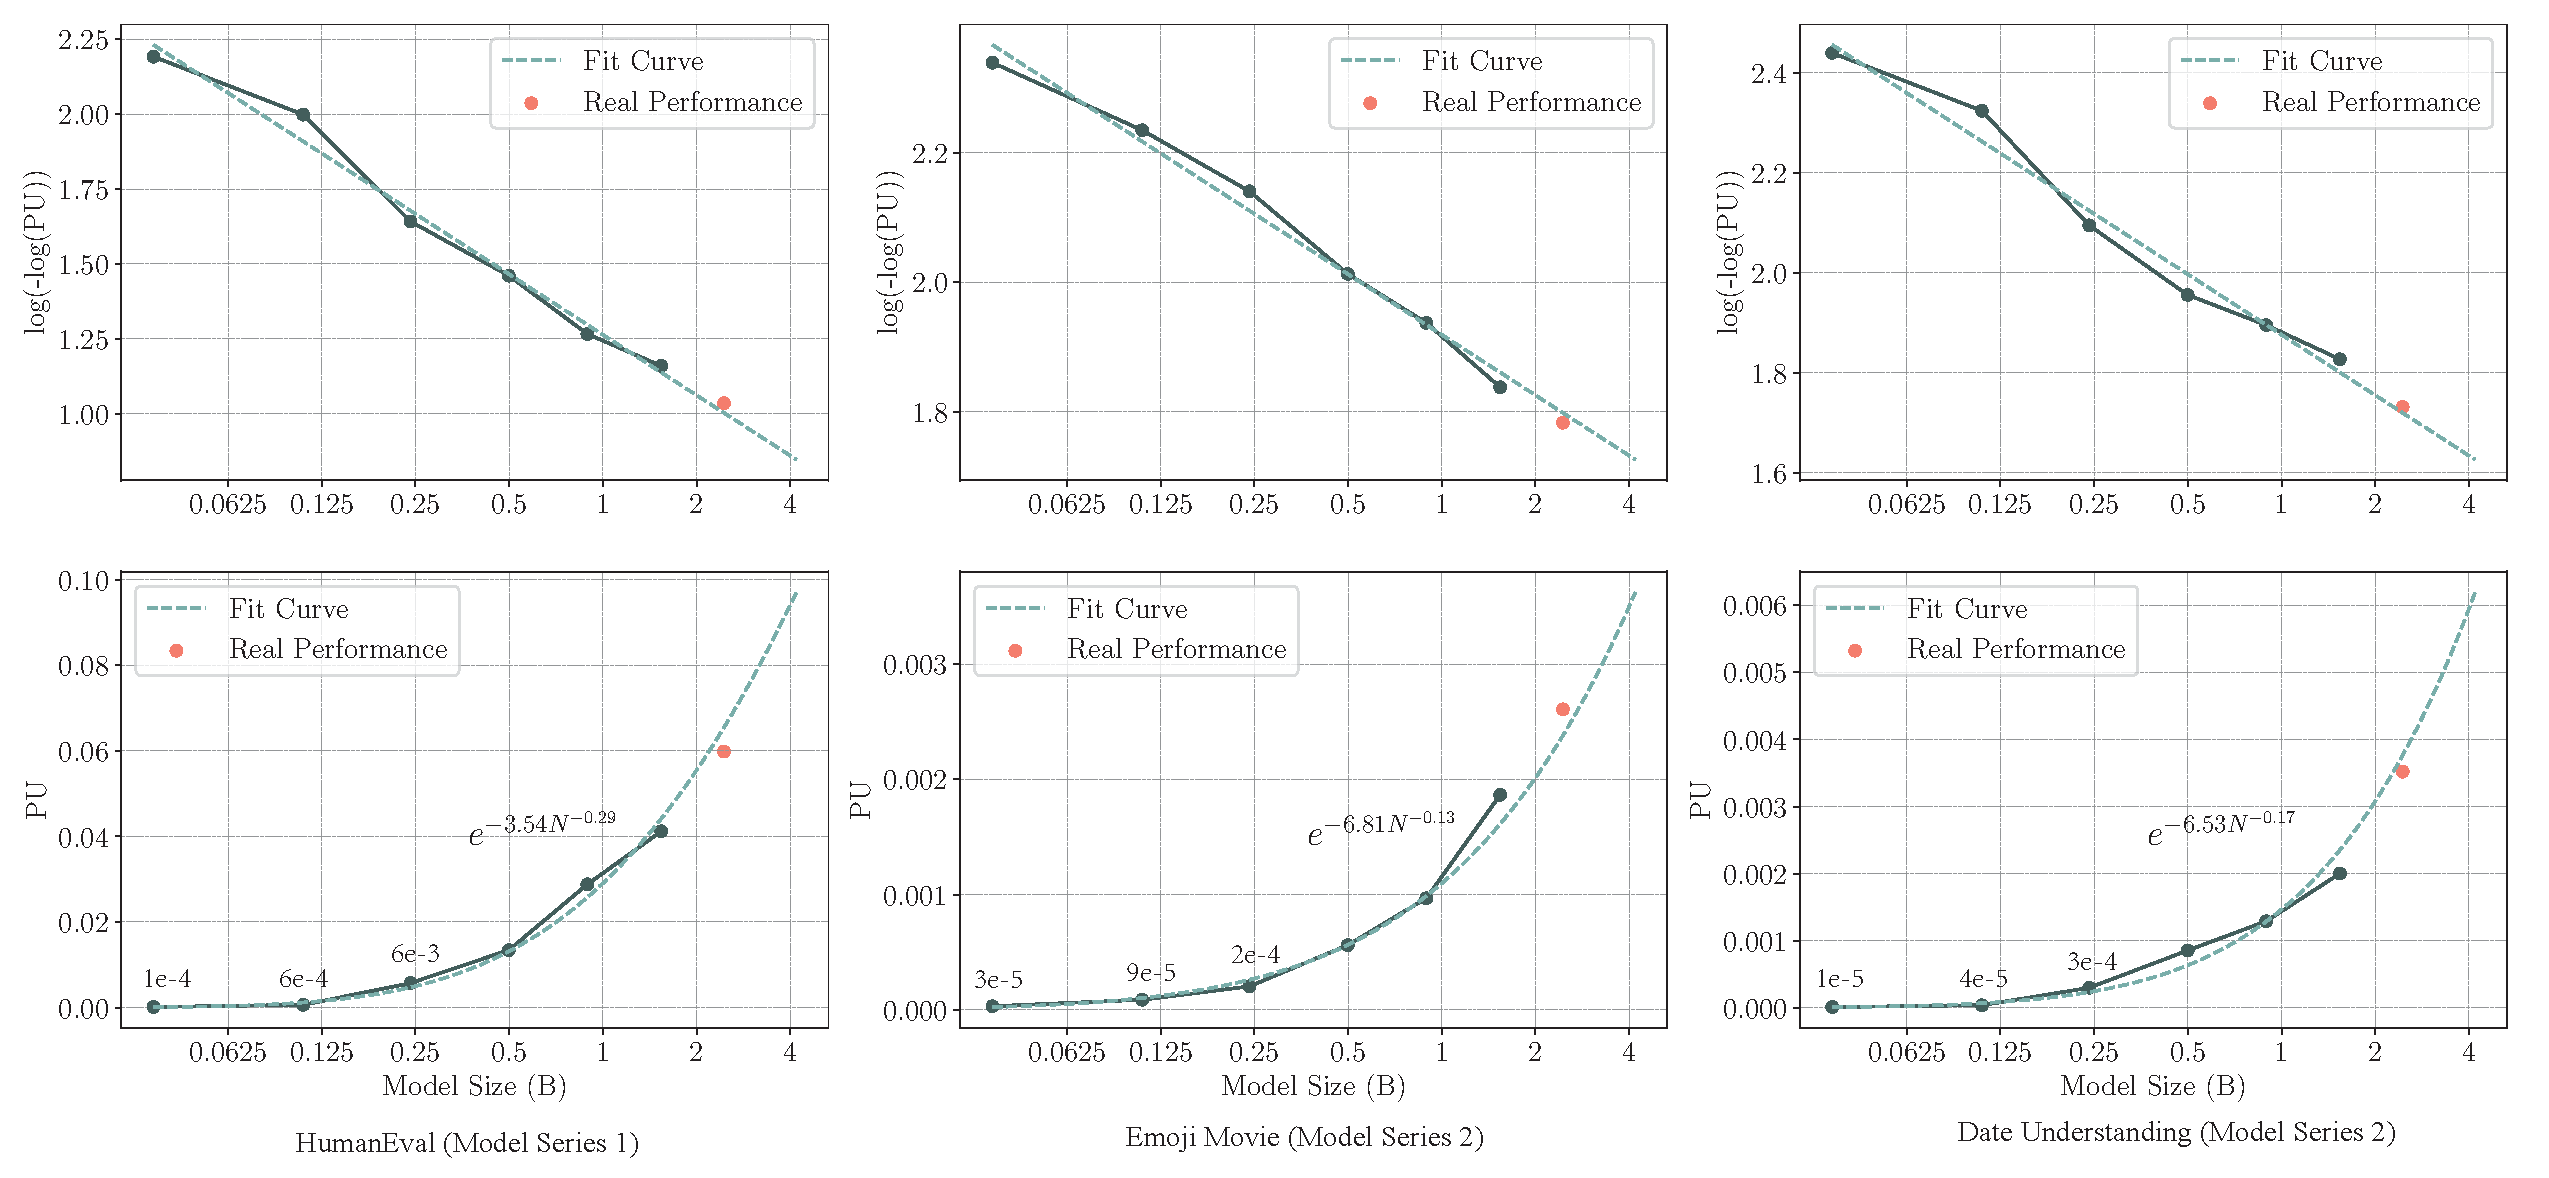
\includegraphics[width=\linewidth]{pufigs/dataset_level_prediction_du.pdf}
        \caption{任务性能随模型规模可预测地扩展。{\color[rgb]{0.85,0.25,0.25}红色}点表示24亿参数模型的实际性能,其与从3000万到15亿参数模型拟合出的任务扩展定律接近。}
    \label{fig:dpu}
\end{figure}

可以观察到,这三个任务在 $\log(-\log(\textsc{PU}))$ 与 $\log(N)$ 之间均呈现出很强的线性关系,从而验证了公式(\ref{eq:task_scaling_raw})所给出的任务扩展定律的有效性。扩展定律函数的估计是利用参数规模从3000万到15亿的模型进行的,利用这些模型对24亿参数模型性能的预测,虽有偏差但在可接受范围内。




\subsection{实例级拟合}

表\ref{tab:easyhardinstances} 展示了HumanEval中一个简单实例和一个具有挑战性实例的“PassUntil”情况。可以观察到,随着模型规模增大,较简单的实例(索引24)呈现出更高的“PU”。然而,更具挑战性的实例(索引20)性能仍然不佳,这表明它们各自的缩放曲线可能存在差异。盲目地对实例的性能进行平均,会使困难实例相对于简单实例的性能提升被掩盖,导致在模型在简单实例上达到饱和后,预测结果不准确。

\begin{table}[h]
    \centering
    \caption{在HumanEval中,简单实例(索引24)相比困难实例(索引20)具有高得多的 $\textsc{PU}$。}
    \begin{tabular}{c|cccccc}
    \toprule
        \multirow{2}{*}{\textbf{实例索引}}  & \multicolumn{6}{c}{\textsc{PassUntil}}   \\
        \cline{2 - 7}
        & \textbf{0.03B} & \textbf{0.1B} & \textbf{0.2B} & \textbf{0.5B} & \textbf{0.9B} & \textbf{1.5B} \\
        \midrule
        20 & 0 & 0 & 0 & 0.000625 & 0.001875 & 0.008125 \\
        % \hline
        24 & 0.00375 & 0.05125 & 0.350625 & 0.3625 & 0.568125 & 0.796875 \\
         \bottomrule
    \end{tabular}
    \label{tab:easyhardinstances}
\end{table}

因此,根据 \ref{sec:instance_level_pass},我考虑了测试样本之间的差异以改进估计。图 \ref{fig:idp_with_modelsize_part1} 中绘制了实例级“PassUntil”的扩展情况。
拟合曲线表明,不同实例的性能不仅起始点不同,而且扩展速度也各异。
尽管如此,它们各自都能通过任务扩展定律进行拟合。部分实例偏离了扩展定律,这有待未来进一步研究。 


\begin{figure}[htbp]
    \centering
    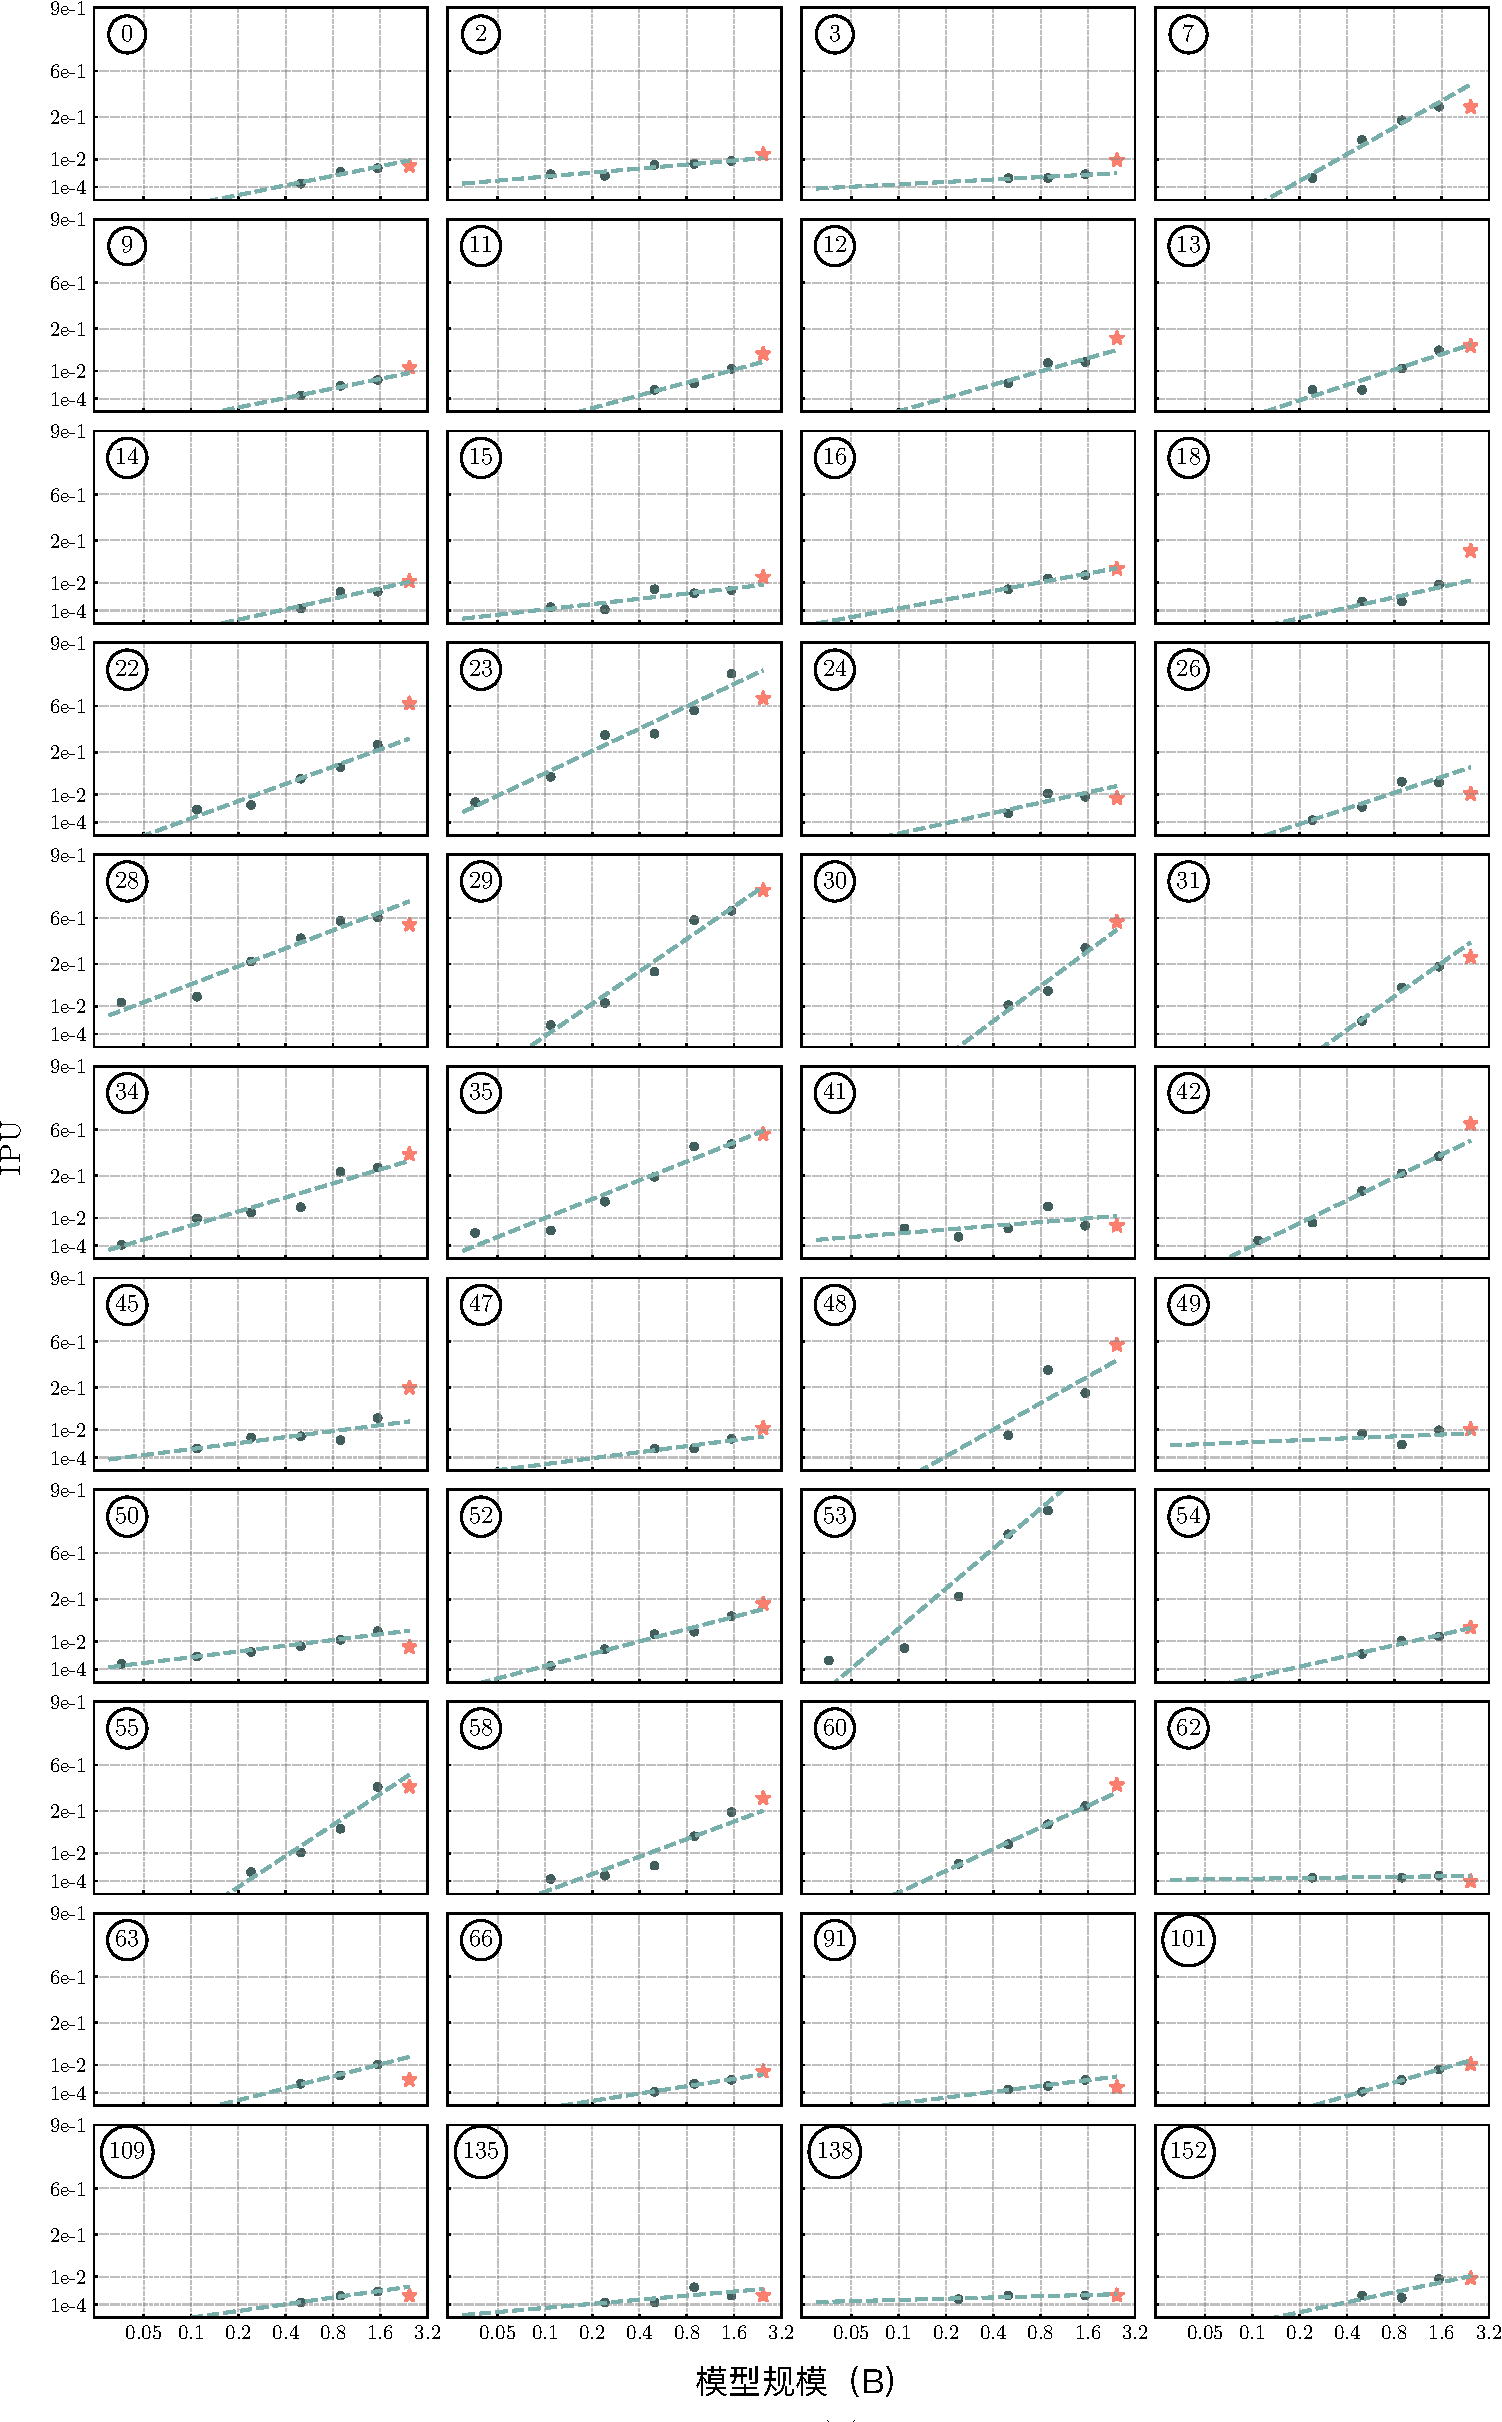
\includegraphics[width=0.85\textwidth]{pufigs/individual_passrate_vs_modelsize_part_main.pdf}
    \label{fig:idp_with_modelsize_part1}
    \caption{实例级扩展定律拟合结果:展示了系列1模型在Humaneval任务上更多单个“PassUntil”扩展曲线的实例。每个子图左上角的标签表示测试集中样本的索引。}
\end{figure}

\begin{figure}[!htbp]
    \centering
    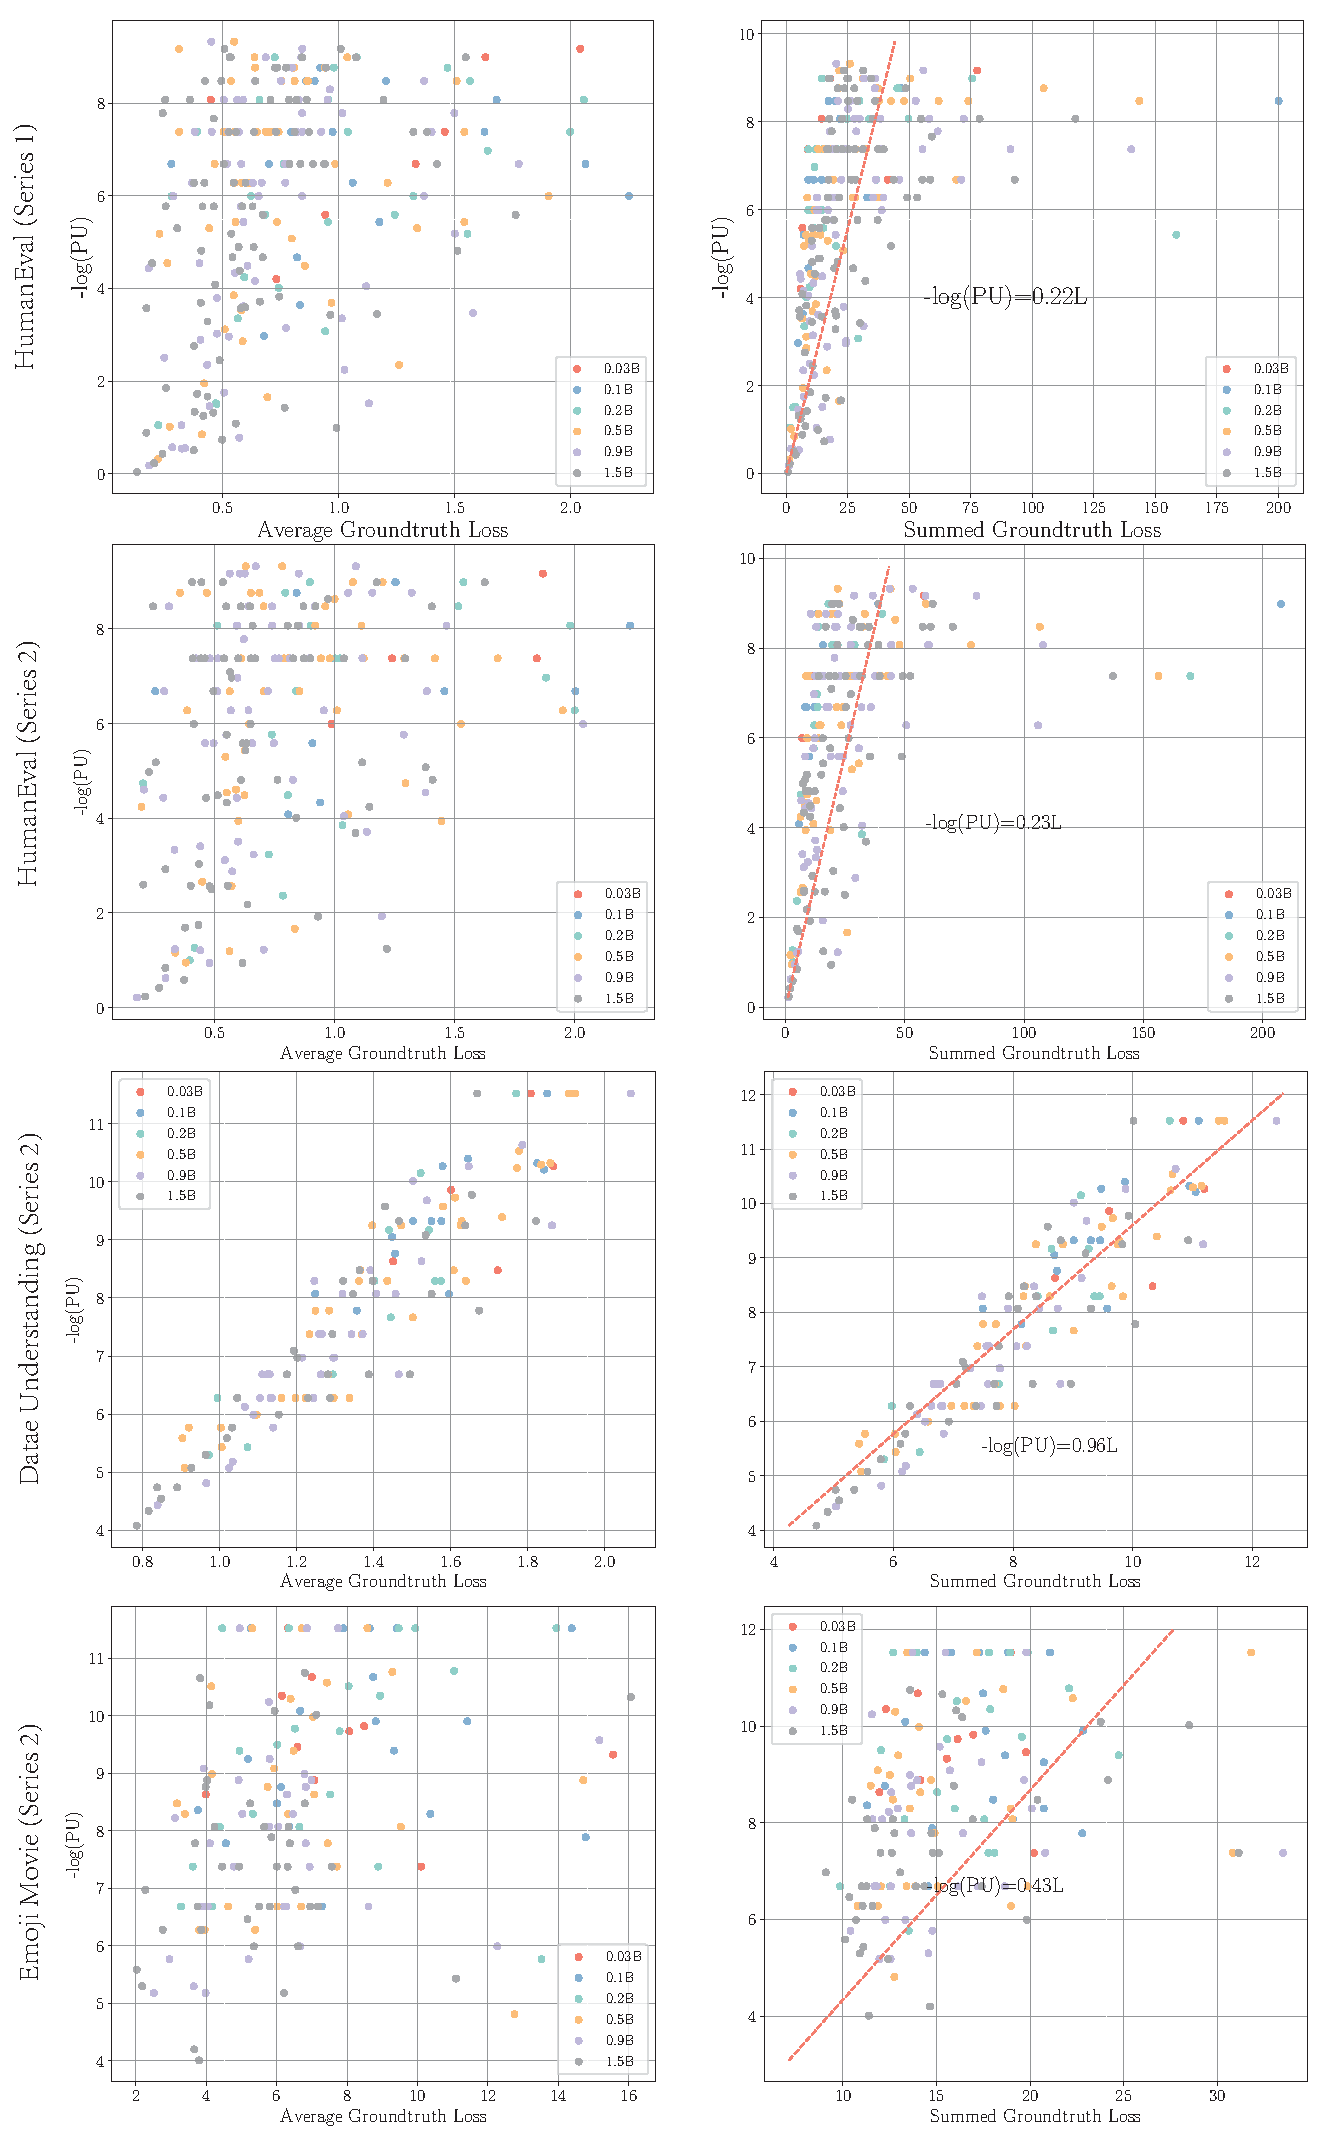
\includegraphics[width=0.8\linewidth]{pufigs/Loss_vs_passuntil.pdf}
    \caption{关于测试损失与“PassUntil”之间关系图。}
\label{fig:loss_vs_passuntil}
\end{figure}

\subsection{从测试损失估计 “PassUntil”}

在实例层面进行估计时,对于难以拟合的实例(即缺乏足够的非零 “PassUntil”值)会面临挑战。随着模型规模的增加,这些样本也可能对 \textsc{PU} 有贡献。因此,本文建议利用真实答案的测试损失来辅助对这类实例的预测。我利用既具有测试损失又有非零 \textsc{PU} 的 “简单” 实例来估计测试损失与 \textsc{PU} 之间的关系(图 \ref{fig:loss_vs_passuntil})。然后,我基于参数规模从3000万到15亿的模型来预测24亿参数模型上每个实例的测试损失。最后,根据上述关系将预测的测试损失转换为预测的 \textsc{PU}。
如图\ref{fig:loss_vs_passuntil}所示,我提出利用真实答案的测试损失来辅助对“困难样本”的预测。对于系列一模型和HumanEval任务,发现其线性关系为\(\textsc{PU} \sim 0.22L\)。对于系列2模型和HumanEval任务,发现线性关系为\(\textsc{PU} \sim 0.23L\)。对于系列2模型和“日期理解”任务,发现线性关系为\(\textsc{PU} \sim 0.96L\)。而对于系列2模型和“表情电影”任务,发现线性关系为\(\textsc{PU} \sim 0.43L\)。 


\begin{table}[!htbp]
    \centering
    \caption{本文任务性能可预测框架的效果:预测值与模型实际性能的预测对比。任务名称后的数字表示评估中使用的模型系列。}
    \scalebox{0.86}{
        \begin{tabular}{lcccc}
            \toprule
            \textbf{方法}  & {\textbf{HumanEval (1)}} & {\textbf{HumanEval (2)}} & {\textbf{Date Understanding (2)}} & {\textbf{Emoji Movie (2)}} \\
            \midrule
            真实值 & 0.05990 & 0.04279 & 0.00346 & 0.002608 \\
            \hline
            数据集层面的拟合 & 0.06550 & 0.05191 & 0.00377 & \textbf{0.002381}\\
            实例层面的拟合 & \textbf{0.05987} & \textbf{0.04402} &\textbf{ 0.00352} & 0.003112\\
            \bottomrule
        \end{tabular}
    }
    \label{tab:final_fit_result}
\end{table}



表\ref{tab:final_fit_result} 中给出了24亿参数模型的最终预测结果,并在图 \ref{fig:final_curve_humaneval_series1} 中绘制预测的 \textsc{PU} 曲线。可以看到,预测结果是准确的,在系列1的HumanEval任务上仅存在0.05\% 的差异,在系列2的 “日期理解” 任务上存在1.7\% 的差异。 


上面使用基于真实标签的损失来辅助“PassUntil”,这可能会引发一种误解:为什么不直接用损失来预测性能呢?下面我详细说明。
\begin{enumerate}
    \item {需要明确区分“损失无法预测任务性能”与“损失有助于预测任务性能”这两种说法。前者指的是在没有其他衡量指标的情况下,仅靠损失不足以用来估计任务性能;而后者表明损失是提高预测准确性的有用因素之一。在本章节中,对这两种说法都进行了明确验证。若不使用“PassUntil”方法,仅从损失值无法推断实际性能(准确率)。例如,损失为1.0并不直接意味着某项任务的准确率为0.2。实际性能必须通过实证测量得到。此外,如图\ref{fig:loss_vs_passuntil}所示,单个样本的损失与“PassUntil”结果并非一一对应,与离散的准确率更是如此。}
    \item {然而,损失确实能提供有用信息。一旦在大量样本集中测量“PassUntil”,就可以建立损失与“PassUntil”之间的统计关系(仅依靠损失数据则无法做到)。这种关系能够提高预测准确性。}
    \item {将损失纳入以改进预测是出于实际考虑,比如计算资源有限,而非必要之举。图\ref{fig:dpu}表明,即使没有损失数据,也能准确预测任务性能。设想一下,如果能够以足够的分辨率测量每个样本,确保每个样本至少通过一次,在这种情况下,损失数据就并非必需。}
\end{enumerate}


\begin{figure}[!htbp]
    \centering
    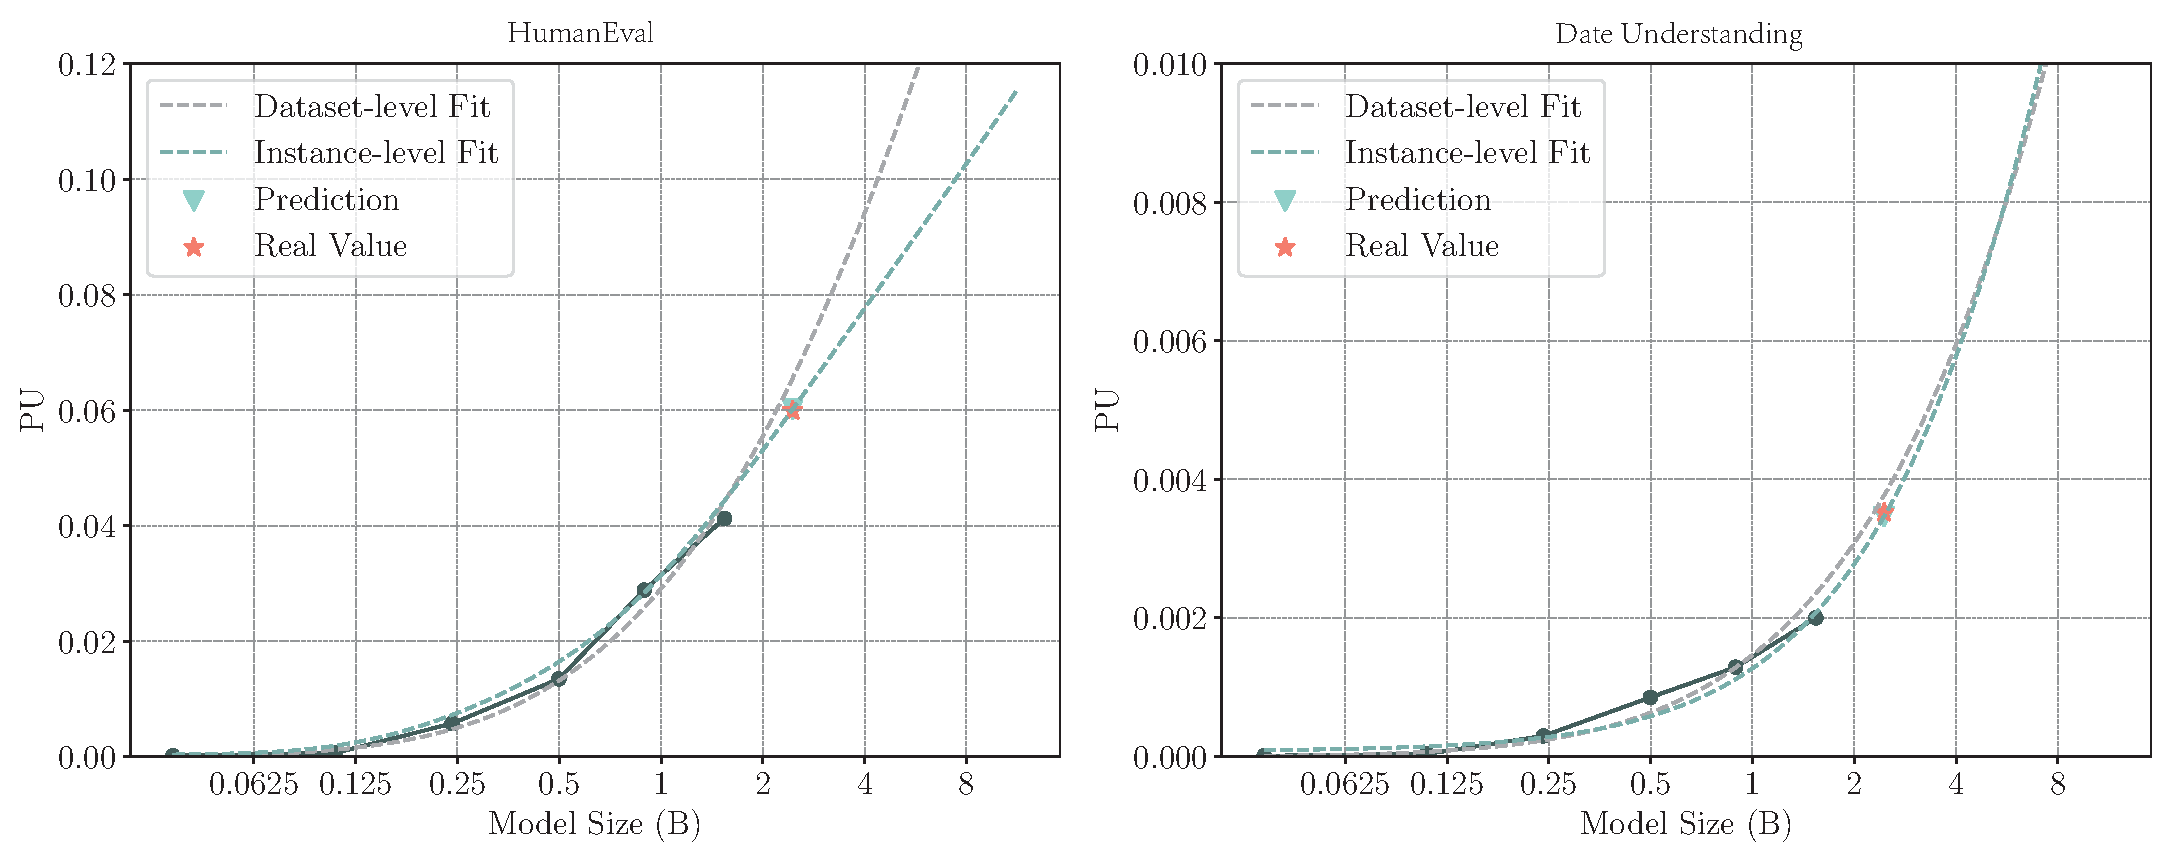
\includegraphics[width=1.02\linewidth]{pufigs/final_predict_2_set.pdf}
    \caption{本文成功预测了24亿参数模型的性能,(左图结果)偏差为0.05\% ,(右图结果)偏差为1.7\% 。 }
    \label{fig:final_curve_humaneval_series1} 
\end{figure}


\section{分析}
\label{sec:emergent}

{基于对任务性能可预测性的发现,我进一步对更广泛任务的扩展行为进行定量分析。我证明,即使有 “PassUntil” 带来的精细分辨率以及其他涌现能力的可预测性,仍有某些能力难以预测。本节给出它们的数学定义,并探讨这种扩展行为可能的解释。}
\begin{figure}
    \centering
        \centering
        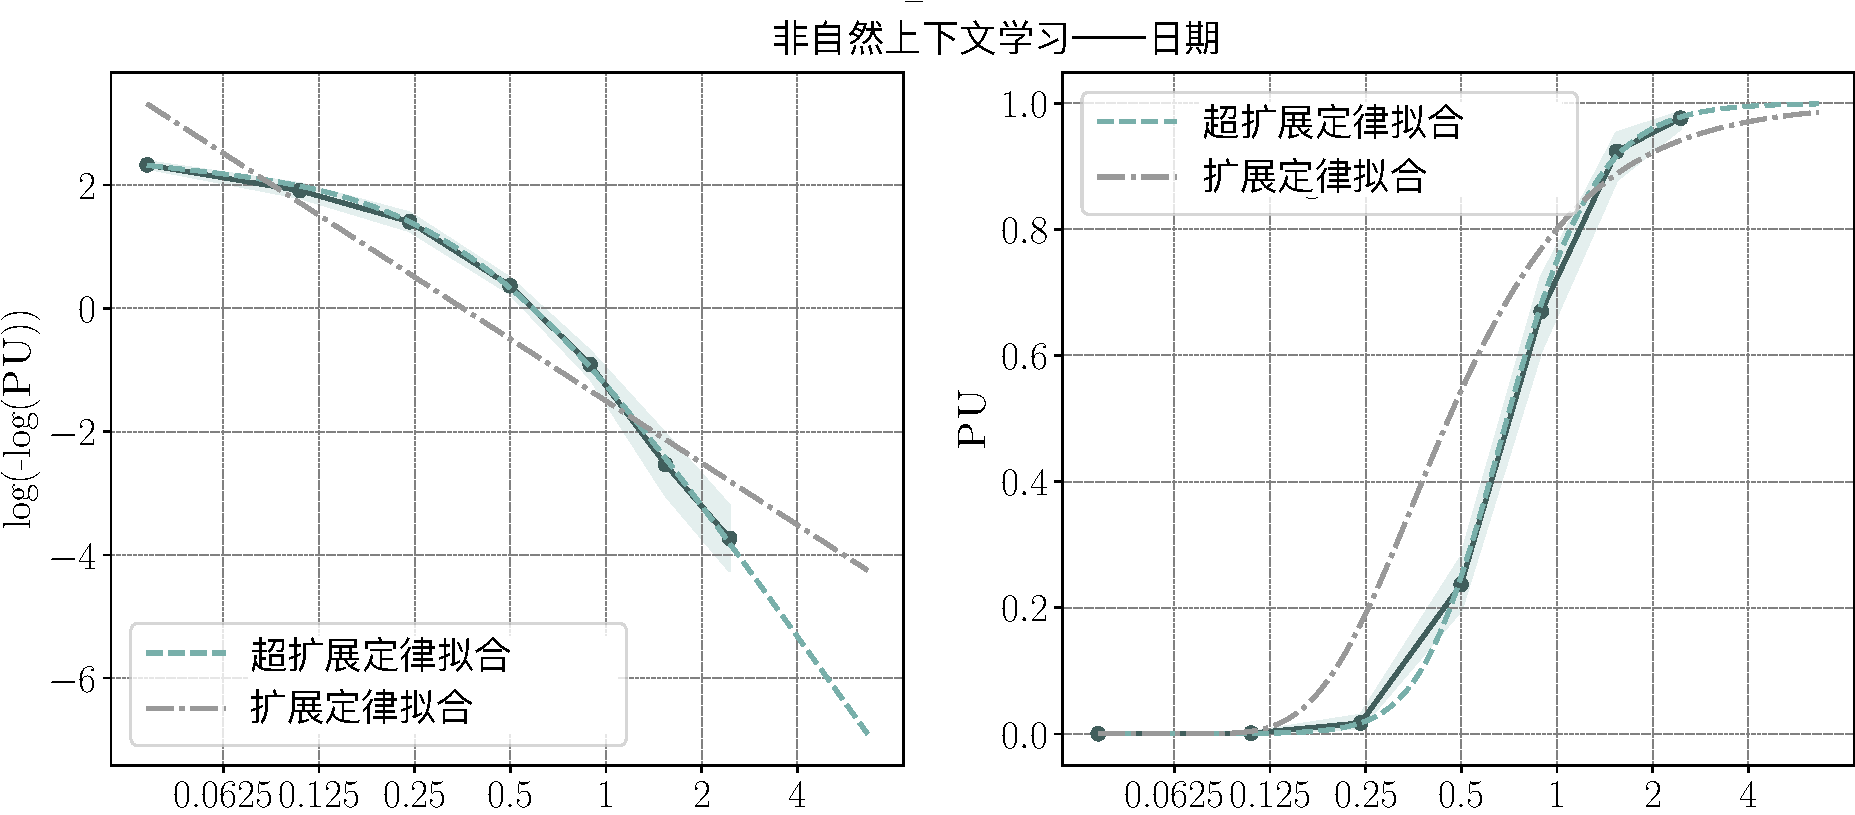
\includegraphics[width=1\linewidth]{pufigs/passrate_vs_modelsize_Dates_circuitfit.py.pdf}
        \centering
\end{figure}
\begin{figure}
        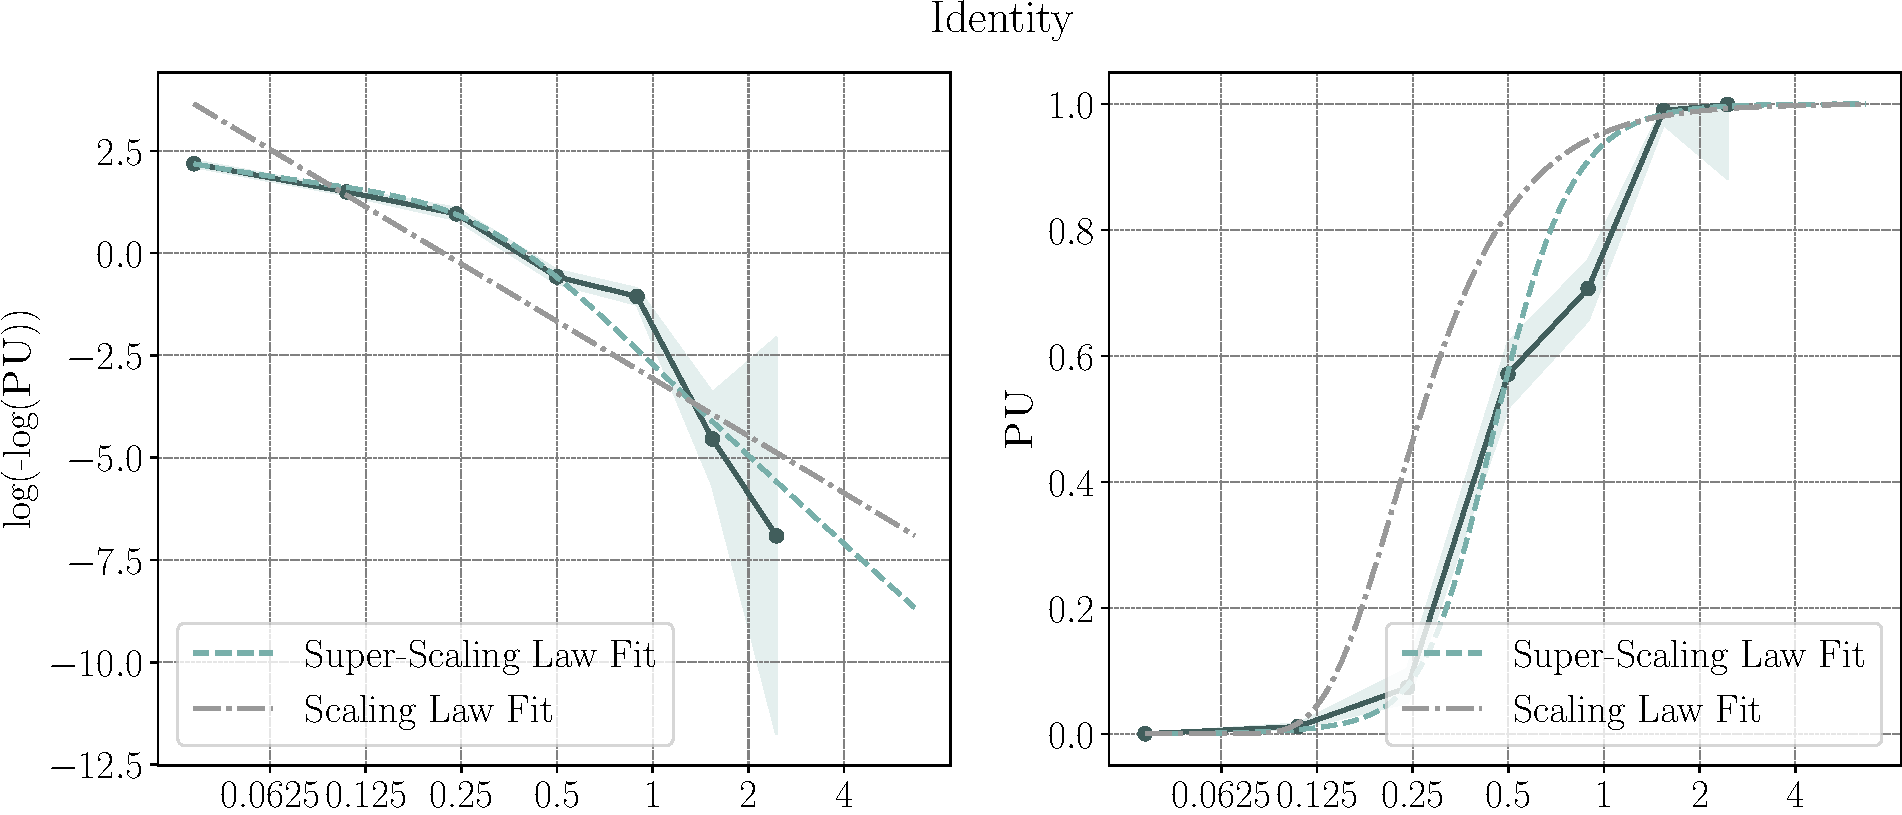
\includegraphics[width=1\linewidth]{pufigs/passrate_vs_modelsize_identity_circuitfit.py.pdf}
        \caption{{“日期”(Dates)和“原样输出”(Identity)任务的扩展曲线。在 $\operatorname{log}(-\operatorname{log}(\textsc{PU}))$ 与 $\operatorname{log}N$ 之间观察到凹函数关系。扩展定律拟合曲线为 {\color[rgb]{0.55, 0.6, 0.6}灰色},超扩展定律拟合曲线为 {\color[rgb]{0.3, 0.6, 0.45}绿色}。}}
        \label{fig:unnatural}
\end{figure}
\begin{figure}å
    \centering
    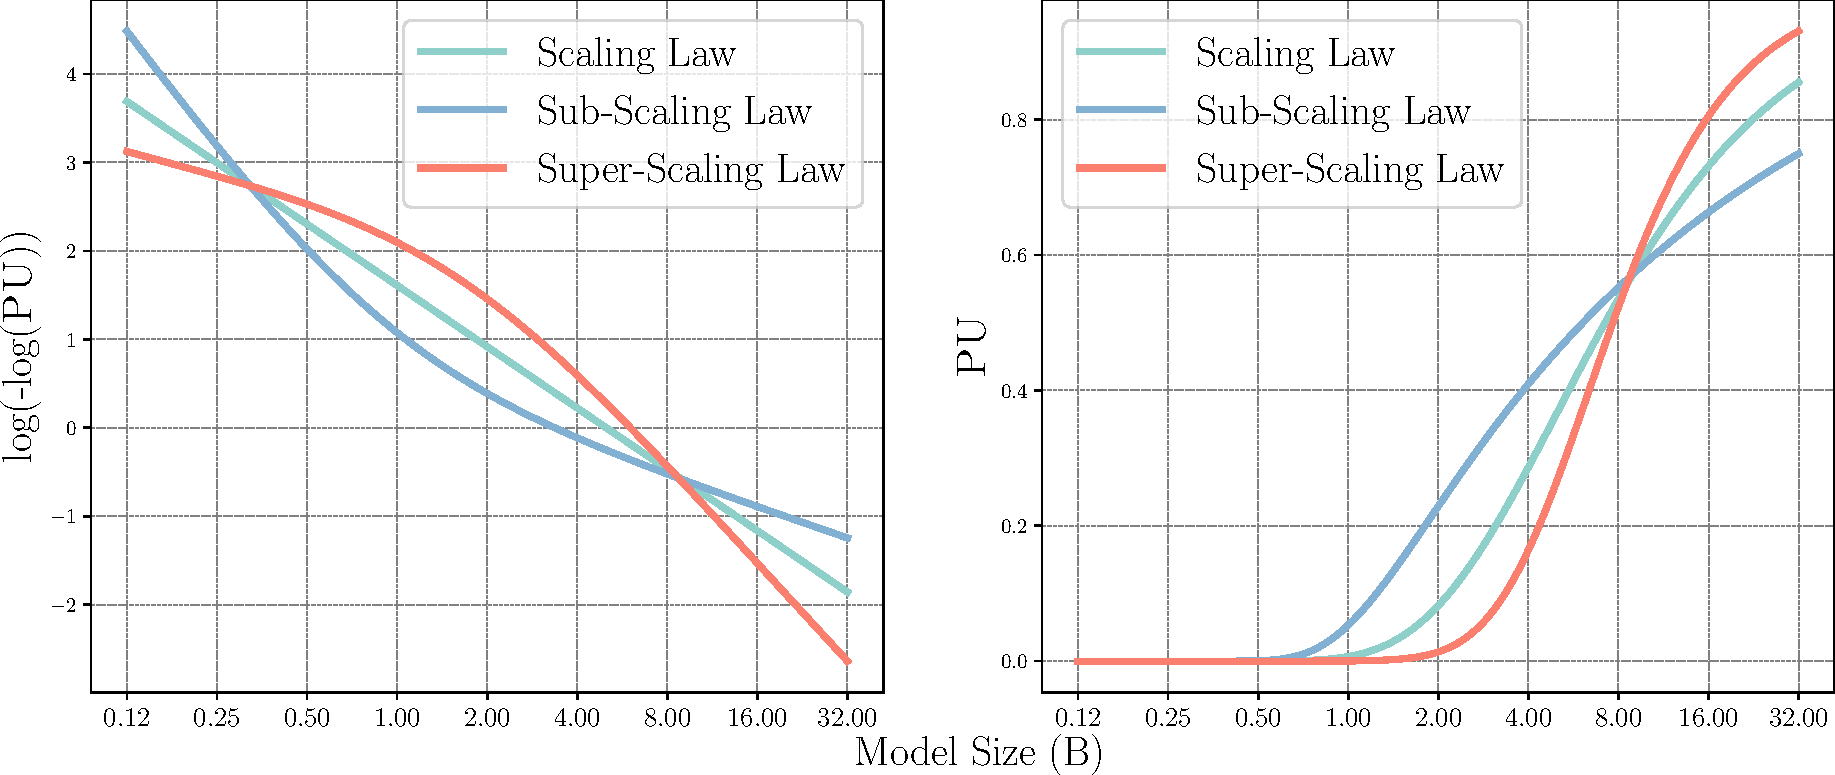
\includegraphics[width=1\linewidth]{pufigs/three_scaling_func.pdf}
    \caption{三种基本的扩展曲线类型,对应于 $\log(-\log(\textsc{PU}))$ 与 $\log N$ 之间的凸函数、线性函数和凹函数。}
    \label{fig:threekindsofgrowth}
\end{figure}

我研究了BigBench\citep{srivastava2022beyond} 中 “非自然上下文学习(UICL)” 类别的扩展曲线。“非自然上下文学习” 包含8个任务,专门用于研究上下文学习能力。这些任务涉及的输入 - 输出对经过有意调整,偏离了典型的训练分布,因此要求模型关注非传统的上下文模式。任务细节和示例见章节\ref{app:unantural_in_context_learning}。在拟合扩展曲线时,仅使用数据集层面的 “PassUntil”,因为这些测试实例是为测试大语言模型的一项技能而人工构建的,可能不存在难度变化。由于测试集较小,我从20个问题的测试结果中进行100次自助采样,并使用自助采样结果计算每个 “PassUntil” 估计值的标准误差(在图中以绿色显示)。 

此外,我展示了非自然上下文学习任务中其余固定子任务的扩展曲线。值得注意的是,图(a)、(b)和(c)中的曲线呈现出凹形模式,即\(\log(\log(-F(N))\)与\(\log N\)之间的关系。具体而言,“两位数”任务呈现出一种有趣的反向扩展趋势,这表明需要进一步研究以明确更清晰的趋势。

{
关于图(d)和(e)中的任务,我观察到这些任务对较小的模型构成重大挑战。具体来说,参数为3000万和1亿的模型未能实现非零通过率,这使得拟合分析的意义不大。此外,对于“反转成自然内容”任务,存在一种明显但轻微的次扩展定律增长趋势。这种趋势可能归因于该任务内在的多步骤特性。
}

\begin{figure}[!htbp]
        \centering
        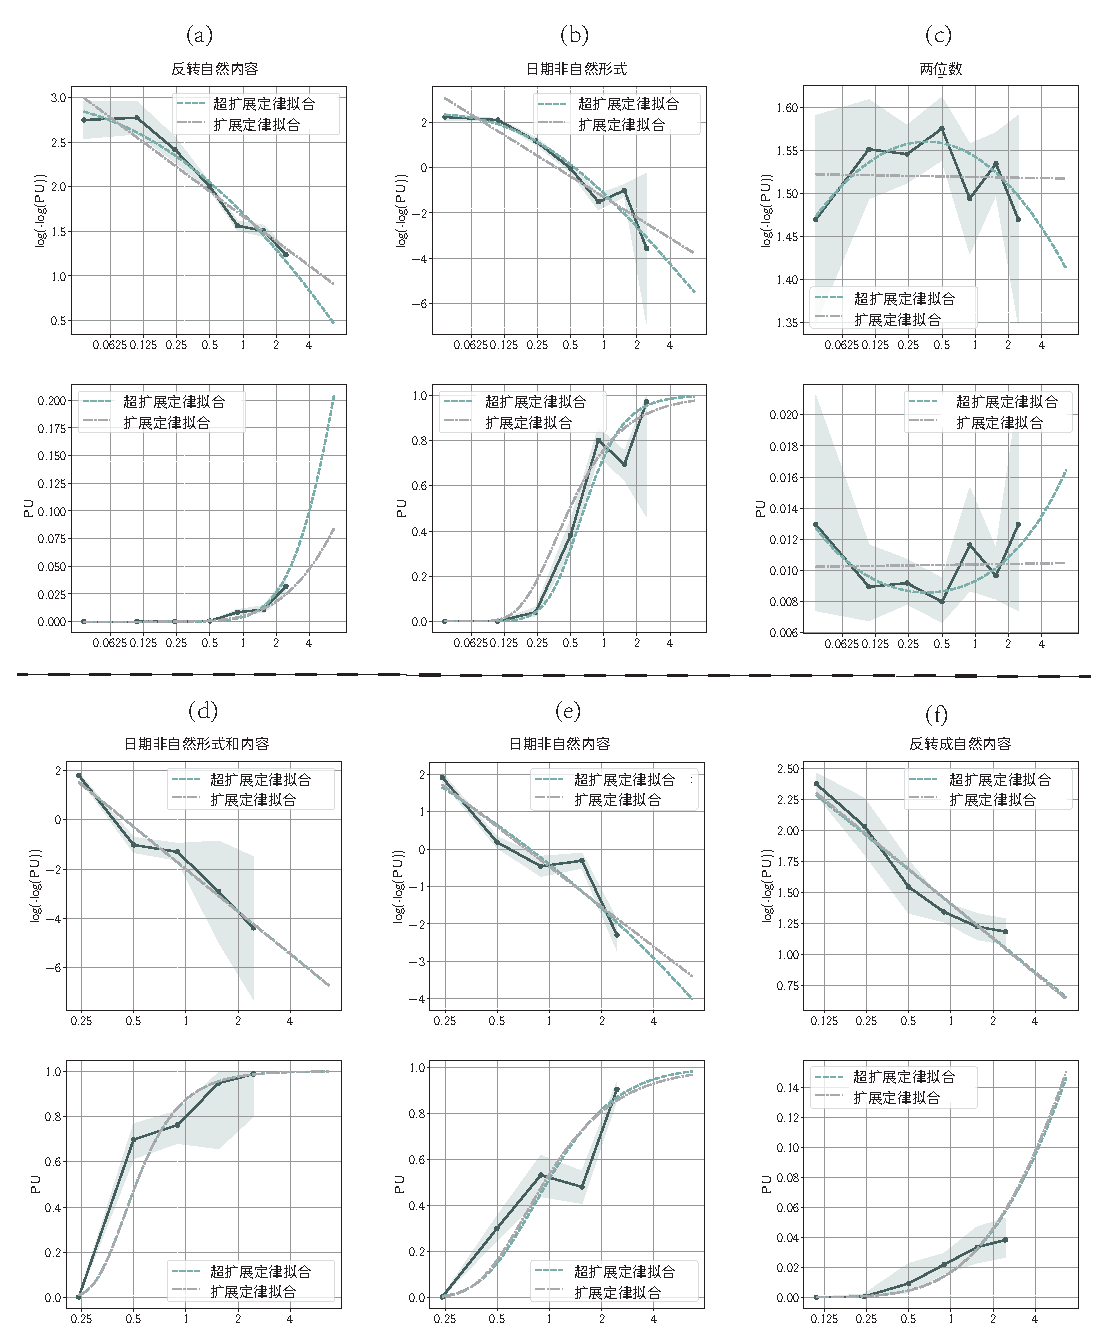
\includegraphics[width=0.9\linewidth]{pufigs/appendix_graph.pdf}
    \caption{{关于非自然上下文学习的补充图。灰色线表示扩展定律拟合,绿色线表示超扩展定律拟合。}}
    \label{fig:appendix_unnatural}
\end{figure}

\subsection{涌现现象的分类}
“日期”(Dates)和“原样输出”(Identity)任务的评估结果如图\ref{fig:unnatural}所示。其他任务见图\ref{fig:appendix_unnatural}。“日期”任务从参数规模3000万开始就呈现出非常平滑且持续的性能提升,而其他任务的提升则略显曲折。尽管如此,这些上下文学习任务中有5/8在\(\log(-\log(\textsc{PU}))\)与\(\log N\)之间呈现出严格的凹函数关系。另外3/8的任务由于对于3000万和1亿参数的模型来说难度极高,缺失了1或2个有效的估计点,因为即使采样\(10^5\)次,“PassUntil”分数仍为0,这留待未来进一步探索。这5/8的任务偏离了扩展定律(公式(\ref{eq:task_scaling_raw})),该定律要求此函数为线性。这意味着,与那些遵循任务扩展定律的任务不同。在遵循任务扩展定律的任务中,“增长速度”\(\alpha\)在不同模型规模下是一致的,而还存在一些任务,随着模型规模增大,其“增长速度”\(\alpha\)会增加。这种现象就是加速涌现现象的例证。为了具体讨论加速涌现现象,先给出任务扩展曲线的分类。

\subsection{涌现现象的数学定义}
由于公式(\ref{eq:loss_scaling_law})的损失扩展定律是模型扩展过程中唯一被广泛接受的原则,本文依据由它推导出来的公式(\ref{eq:task_scaling_raw})的任务扩展定律,来区分涌现现象和其他扩展行为。

% \newtheorem{definition}{定义}

对于一系列模型,设非嵌入参数的数量为变量\(N\),假设在某一任务上通过“PassUntil”估计得到的\(\textsc{PU}(N)\)是\(N\)的连续函数。定义\(F(N) = \operatorname{log}(-\operatorname{log}(\textsc{PU}(N)))\),{那么一个任务的扩展曲线可分为三个基本主要类别\footnote{如果\(F(N)\)同时有凸函数和凹函数部分,那么可称其为混合增长。}:}
\begin{enumerate}
    \item 如果\(F(N)\)是\(\operatorname{log}N\)的线性函数,那么该任务遵循扩展定律增长。
    \item 如果\(F(N)\)是\(\operatorname{log}N\)的凸函数,那么该任务遵循次扩展定律增长。
    \item 如果\(F(N)\)是\(\operatorname{log}N\)的凹函数,那么该任务遵循超扩展定律增长,即“加速涌现”。
\end{enumerate}


图\ref{fig:threekindsofgrowth}展示了这三种增长类型的可视化结果。定性地看,当性能开始显著提升时,这三种类型的扩展曲线都类似于指数增长。然而,它们在性质上是不同的。遵循任务扩展定律增长或次扩展定律增长的任务扩展曲线更容易预测和控制,而加速涌现则不易预测,并且随着模型规模增大可能会失控。

{\textbf{扩展曲线形状的成因}。上述数学定义为本文提供了检验关于这些扩展行为成因假设的机会。在此,我首先研究以下假设:涌现能力可能由多步推理引发\citep{srivastava2022beyond, wei2022emergent, schaeffer2023emergent}。}

我证明了\textbf{”多步推理会导致次扩展定律增长”}。

\begin{theorem}
假设每个推理步骤的成功率(通过“PassUntil”衡量)遵循扩展定律增长,那么多步推理的成功率遵循次扩展定律增长。
\end{theorem}


    
\begin{proof}
    假设推理步骤\(i\)的“PassUntil”分数(\(\textsc{PU}\))遵循具有系数\(c_i\)和\(\alpha_i\)的扩展定律增长,总体成功率为:
    \begin{equation}
    \begin{split}
     F(N) & = \operatorname{log}\left(-\operatorname{log}\prod_i P_i\right)\\ & = \operatorname{log}\left(-\operatorname{log} \prod_i\operatorname{exp}\left(- c_i \operatorname{exp}(-\alpha_i \operatorname{log} N)\right)\right) \\ & = \operatorname{log}\left(\sum_i c_i \operatorname{exp}\left(-\alpha_i \operatorname{log} N \right)\right)\\
    \end{split}
    \end{equation}
    然后对\(F(N)\)关于\(\log N\)求二阶导数,可得:
    \begin{equation}
    \label{eq:app_th_1}
    \begin{split}
        \frac{\partial^2{F}}{\partial{(\operatorname{log}N )^2}} & = \frac{\sum_i \alpha_i^2 c_i \exp(-\alpha_i \log N) \sum_i c_i \exp(-\alpha_i \log N)}{(\sum_i c_i\exp(-\alpha_i \log N))^2} \\
    & - \frac{(\sum_i \alpha_i c_i \exp(-\alpha_i \log N) )^2}{(\sum_i c_i\exp(-\alpha_i \log N))^2}
    \end{split}
    \end{equation}
    令\(k_i = c_i \exp(-\alpha_i \log N) > 0\),式(\ref{eq:app_th_1})变为:
    \begin{equation}
    \frac{\sum_i \alpha_i^2 k_i\sum_i k_i - (\sum_i \alpha_i k_i)^2}{(\sum_i k_i)^2}
    \end{equation}
    利用柯西 - 施瓦茨不等式,可以证明:
    \begin{align}
    \frac{\partial^2{F}}{\partial{(\operatorname{log}N )^2}} \geq 0, \quad \forall  \alpha_i > 0, c_i > 0
    \end{align}
    只有当\(\frac{\alpha_i \sqrt{k_i}}{\sqrt{k_i}} = \text{常数}\)时,等式成立,即推理链中的所有步骤以相同速度扩展时。
    因此,\(F(N)\)是\(\operatorname{log}N\)的凸函数,且扩展曲线呈现次扩展定律增长。 
\end{proof}


这个证明也可以更直观地理解:增长速度最初会受到那些简单步骤改进的推动,最终会受到最困难步骤的限制,从而呈现出增长速度下降的趋势。

我提出另一种假设:根据\citet{elhage2021mathematical},大语言模型中可能存在多个神经“回路”,只要其中一个回路能够成功解决测试实例,就认为该测试实例通过。这个假设的灵感来自于\cite{varma2023explaining}对“顿悟”现象的解释。他们提出在Transformer内部存在一个记忆回路和一个泛化回路,“顿悟”现象是由于在训练过程中泛化回路比记忆回路效率更高所导致的。我将证明,基于这个假设,扩展曲线会呈现出涌现的特征。

\begin{theorem}
假设大语言模型中存在多个负责解决任务的回路\(i\),每个回路都呈现扩展定律增长且有\(\textsc{PU}_i\)。{并且假设}任务的成功率是这些回路的多数表决结果,即\(F(N)  = \operatorname{log}\left(-\operatorname{log}\max_i \textsc{PU}_i\right)\)。
那么,\(F(N)\)是\(\operatorname{log}N\)的凹函数。
\end{theorem}

\begin{proof}
    \begin{equation}
    \label{eq:app_th_2}
    \begin{split}
    F(N) &= \operatorname{log}\left(-\operatorname{log}\max_i \operatorname{exp}\left(- c_i \operatorname{exp}(-\alpha_i \operatorname{log} N)\right)\right) \\
        &= \operatorname{log} \min_i  c_i \operatorname{exp}(-\alpha_i \operatorname{log} N) \\
    &=  \min_i (\operatorname{log} c_i-\alpha_i \operatorname{log} N) \\
    \end{split}
    \end{equation}
    由于取最小值操作保持凹性,所以\(F(N)\)是\(\operatorname{log}N\)的凹函数。 
\end{proof}


我通过拟合UICL任务的扩展曲线对该假设进行了初步检验。在实际操作中,与\cite{varma2023explaining}类似,我采用了一种软多数表决版本。我在两个回路之间应用加权组合。并且假设回路数量为\(2\)。因此,用\({w_1}({\alpha_1}\log N-\log{c_1}) + {w_2}({\alpha_2}\log N - \log c_2)\)来拟合\(F(N)\),其中\(w_1\)和\(w_2\)由\({\alpha_i}\log N -\log {c_i}\)的Softmax函数给出。得到的拟合曲线在图\ref{fig:unnatural}和图\ref{fig:appendix_unnatural}中以{\color[rgb]{0.3, 0.6, 0.45}绿色}线条展示。可以看到,这个假设得到的拟合曲线与观察到的性能扩展曲线更为吻合。 



\section{本章小结}

本章引入了一种全新的评估策略,该策略能够检测模型在规模缩放过程中极其微小的性能提升,从而为定量衡量任务扩展定律和涌现能力开辟了道路。借助这种方法,我成功预测了更大规模模型的任务性能。此外,对涌现能力进行了定量分析,从而更清晰地洞察扩展过程中不可预测因素的本质和起源。这项研究不仅加深了我对大语言模型(LLMs)缩放特性的理解,也为未来大语言模型可预测的规模化扩展研究奠定了基础。 